% \chapter{Jointless Bridges}\label{chp:jointless-bridge}
\chapter{无缝桥梁}
\label{chp:jointless-bridge}
% \section{Introduction}
\section{简介}
% A jointless bridge has a continuous deck with no expansion joints over the superstructure, abutments, and piers, and is also commonly referred to as an integral bridge. In this type of bridge structure, all movement due to thermal, creep, and shrinkage strain is accommodated either within the system itself or at the ends of the approach slabs where the slabs abut the roadway pavement. Because there are no joints, ride quality is improved and maintenance can be greatly reduced.
无缝桥具有连续桥面,在上部结构、桥台和桥墩上没有伸缩缝,通常也称为整体桥。在这种类型的桥梁结构中,由于热应变、徐变应变和收缩应变引起的所有运动要么在系统本身内,要么在引道板与车行道路面相邻的端部进行调节。由于没有接头,乘坐质量得到提高,维护工作也大大减少。

% Leaking deck joints have been a major cause of bridge deterioration and reduced service life, especially where roadway drainage carrying deicing chemicals can spill onto bridge elements below. Elimination of bridge deck expansion joints is therefore an important consideration in bridge system selection to provide long-term service life, as discussed in \cref{chp:bridge-system-selection}.

桥面接缝漏水一直是桥梁劣化和使用寿命缩短的主要原因,尤其是在道路排水系统中,携带除冰化学品的排水系统可能会溢出到下方的桥梁\gls{element}上。因此,如\cref{chp:bridge-system-selection}所述,消除桥面伸缩缝是选择桥梁系统以提供长期使用寿命的重要考虑因素。

% This chapter provides a summary of design, construction and maintenance provisions related to the use of jointless bridges.
本章概述了与使用无缝桥梁相关的设计、施工和维护规定。

\section{History of Jointless Bridges}
A detailed history of jointless bridges is provided by Burke, Jr. (2009). On the basis of a nationwide mail survey of state and province transportation departments, it appears that the Ohio highway department was one of the first agencies to initiate the routine use of continuous construction for multi-span bridges (Burke, Jr. 2009). However, these bridges had expansion joints at abutments. Ohio began this practice in 1930.

In conjunction with the development and adoption of continuous construction for all moderate length highway bridges, Ohio Department of Transportation (DOT) was also the first to routinely eliminate deck joints at abutments. The first integral bridge in the United States was the Teens Run Bridge. It was built in 1938 near Eureka in Gallia County, Ohio, and consisted of five continuous reinforced concrete slab spans supported by capped pile piers and abutments. Since that time, construction of integral bridges has spread throughout the United States and abroad. The United Kingdom recently adopted them for routine applications, Japan completed its first two in 1996, and South Korea completed its first such bridge in 2002.

The Tennessee DOT now is leading the way in construction of continuous bridges. For example the Long Island bridge of Kingsport was constructed in 1980 using 29 continuous spans without a single intermediate deck expansion joint.

Continuous integral bridges with steel main members have performed successfully for years in the 300 ft range in such states as North Dakota, South Dakota, and Tennessee. Continuous integral bridges with concrete main members 500 to 800 ft long have been constructed in Kansas, California, Colorado, and Tennessee.

As of 1987, 11 states reported building continuous integral bridges in the 300 ft range. Missouri and Tennessee reported even longer lengths. Missouri reported steel and concrete bridges in length of 500 and 600 ft respectively. Tennessee reported lengths of 400 and 800 ft for similar bridges. Sixty percent of those departments responding to the 1987 survey were using integral construction for continuous bridges.

More recently, the Tennessee DOT completed the Happy Hollow Creek Bridge, a seven-span prestressed concrete curved integral bridge with a total length of over 1175 ft. In that bridge, tall flexible twin circular column piers support the superstructure. A single row of steel H-piles is used to support each abutment. Although to some engineers the length of this structure may seem extreme, it is well within the Tennessee DOT’s bridge design policy statement regarding the length of integral bridges.

Seamless bridges are another type of jointless bridges introduced by SHRP 2 R19A for practice in the United
States, which allows elimination of expansion joints even at the end of the approach slab. The seamless bridge system
was first introduced by Russell Bridge et al. (2000) in Australia for use with continuously reinforced concrete
pavement for the approach roadways. Most commonly used pavements in the United States, however, are jointed
plain concrete (JPCP) and flexible pavements, which require a modified application. Seamless bridges do not have
any joints, even at the ends of an approach slab (hence seamless). Instead, a pavement transition zone is used to
dissipate the thermal displacements of the bridge. The transition zones can be rather lengthy relative to the bridge. The
benefit however, is that movements at the end of the transition zone are very small.

\section{Types of Jointless bridges}
Three main types of jointless bridges are described in this chapter: integral and semi-integral jointless bridges,
which are commonly used in practice, and a new class of jointless bridges, referred to as seamless jointless bridges.
The main characteristic of the seamless system is that expansion joints are eliminated altogether and the bridge deck is
connected to the approach road pavement with no joint.

\cref{fig:jointless-element} shows a rendering of a typical layout of a jointless bridge, shown with the superstructure cast in an integral abutment.

\begin{figure}
  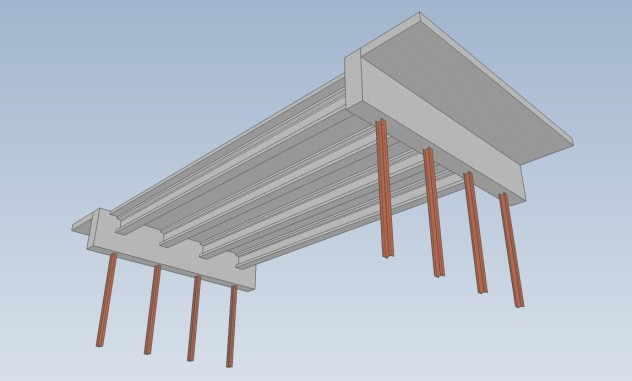
\includegraphics[height=4.5cm]{jointless-element1.jpg}
  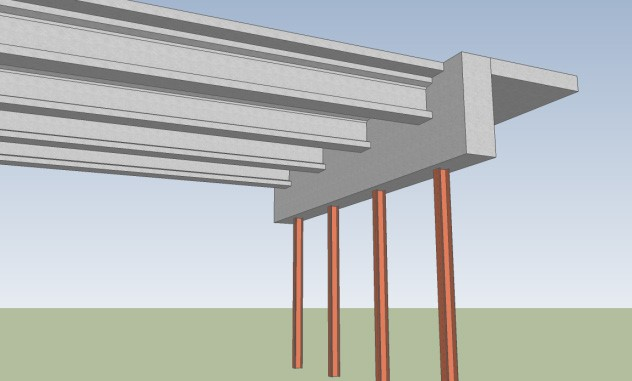
\includegraphics[height=4.5cm]{jointless-element2.jpg}
  \caption{无缝整体桥的\gls*{element}}
  \label{fig:jointless-element}
\end{figure}

\subsection{Integral Bridges}
Integral bridges have superstructure constructed monolithically with the abutments, encasing the ends of the
superstructure within the backwall. The main characteristics of integral bridges are their jointless construction and
flexible abutment foundations. The system is structurally continuous and the abutment foundation is flexible
longitudinally. The movement of the superstructure is accommodated by the foundation.

\cref{fig:jointless-element} shows, schematically, the main elements of an integral bridge system, which consist of bridge deck,
girders, integral cast abutments, and approach slabs. The bridge movement is accommodated at the ends of the
approach slabs. Also, sleeper slabs are commonly used to provide vertical support for the ends of the approach slab
where the slabs abut the roadway pavement (not shown in \cref{fig:jointless-element}). In addition, jointless integral bridges can be
continuous multi-span structures with intermediate piers (also not shown in \cref{fig:jointless-element}). Various details are described
in greater detail in Section 8.7, which also includes further discussion of sleeper slabs in Section 8.7.3.

\subsection{Semi-Integral Bridges}
Semi-integral bridges are defined as having an end diaphragm serving as the abutment backwall and that is cast encasing the superstructure ends. In this system, the superstructure rests on expansion bearings and the end diaphragm is not restrained longitudinally with respect to the pile cap or abutment stem. The deck may be sliding, or cast monolithically with the backwall, but does not have a joint above the abutment. The foundation is rigid longitudinally,
where superstructure movement is accommodated through bearings.

The main elements of a semi-integral bridge system consist of bridge deck, girders, abutment stem and bearing
seat, integral cast diaphragm backwall, approach slab, and sleeper slab. The bridge movement is accommodated at the
ends of the approach slabs. Greater detail is provided in in Section 8.7.


\subsection{Seamless Bridges}
The seamless bridge system is characterized by eliminating the need for expansion joints, even at the ends of the
approach slabs, while limiting the longitudinal expansion and contraction of the bridge superstructure. Imposing the
limitation on longitudinal expansion and contraction of the bridge superstructure results in development of
longitudinal forces that need to be resisted with appropriate design features. It should be noted that longitudinal
expansion and contraction is limited, but not eliminated. This philosophy is used to reduce the level of longitudinal
forces that can be developed, while making the gap between end of transition zone and start of pavement manageable
(to less than about 0.25 in.). The foundation requirements are very similar to those of integral abutments. A seamless
bridge system for jointed pavement types used in the United States was developed by SHRP 2 R19A project and
described in Appendix E. Additional information on this system can be found in Ala (2011), as well as in Ala and
Azizinmanini (2013a, 2013b).

\cref{fig:seamless-bridge} shows, schematically, the main elements of the seamless bridge system developed by SHRP 2 R19A
(Ala 2011; Ala and Azizinamini 2013a; Ala and Azizinamini 2013b). The main elements of the system consist of
bridge deck, transition zone and roadway pavement. The bridge movement is accommodated within the transition
zone, and the movement at the end of the transition zone is relatively small. This eliminates having expansion joints at
the end of transition zone, where the roadway pavement starts. The thickness of the transition zone and approach slab
near the abutment is increased to account for lack of support from soil below. The assumption is that the transition zone near the abutment has no support and resists the imposed loads by flexure. Appendix E provides detailed
information about this new system.

\begin{figure}
  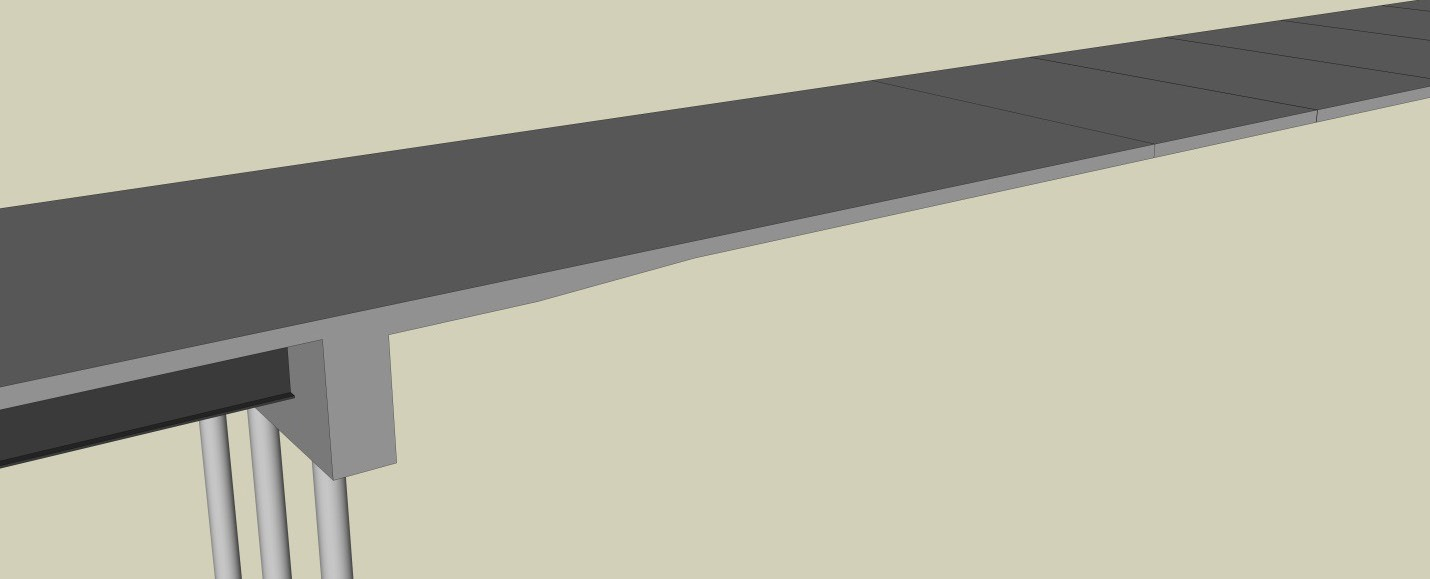
\includegraphics[width=\linewidth]{seamless-bridge.jpg}
  % \caption{Seamless bridge system}
  \caption{Seamless bridge system}
  \label{fig:seamless-bridge}
\end{figure}

\subsection{Advantages of Jointless Bridges}
\pnme{Henry Derthick}, former engineer of structures at the Tennessee DOT, once stated, “The only good joint is no joint.” In keeping with this statement, known advantages of the jointless bridge systems include:

\begin{itemize}
  \item Lower initial cost,
  \item Lower maintenance cost,
  \item Prevention of leakage of moisture to bridge elements below deck resulting in longer service life,
  \item Improved ride quality,
  \item Easier and faster construction,
  \item Easier inspection,
  \item Simplified bridge details,
  \item Elimination of bearings (except for semi-integral),
  \item Ideally suitable for bridges with skew and curvature or located in high seismic areas, and
  \item Enhanced buoyancy resistance of the bridge.
\end{itemize}

Because of these advantages, many DOTs have started using jointless bridges; however, the design provisions vary significantly from one state to another.

\subsection{Cost Effectiveness of Jointless Bridges}

Jointless bridges have a significant cost savings advantage as compared to traditional bridges with expansion
joints. As mentioned, cost savings are realized both during initial construction and throughout the life of the bridge
with reduced maintenance. This is particularly true for bridges with integral abutments.

Most components of typical bridges with joints and jointless bridges are similar in construction and cost (deck,
beams, cross frames, etc.). Thus, a comparison is made relative to the different components that distinguish each type
of construction (e.g., the costs of the abutments and expansion joints). In addition, since unit pricing of each item is
neither consistent from region to region nor over time, a qualitative comparison is made using relative costs.

It is recognized that different states and municipalities have different specifications and construction techniques;
however, initial construction of a typical abutment with an expansion joint will most often include the following:

\begin{itemize}
  \item Excavation;
  \item Two rows of piling (in some cases);
  \item Concrete cap, stem, diaphragm, and backwall with reinforcing (three pours);
  \item Elastomeric bearings, per beam;
  \item Precision-cast bridge seats for bearings;
  \item Expansion joint; and
  \item Porous backfill.
\end{itemize}

Similarly, typical construction of an integral bridge includes:

\begin{itemize}
  \item Excavation;
  \item One row of piling;
  \item Concrete cap, integral backwall, and diaphragm (two pours);
  \item Sleeper slab with reinforcement; and
  \item Porous backfill.
\end{itemize}

The important differences between an integral abutment and a traditional abutment with a jointed deck include a
lack of expansion joint, no bearings, reduced number of required piles, reduced number of concrete pours, and
inclusion of a sleeper slab. Taking these differences into consideration, the cost savings are readily apparent. The
sleeper slab adds a few cubic yards of concrete and an extra detail to the cost, but removal of the expansion joint,
removal of the second row of piling (overall reduced number of piles), reduction in the required concrete and
reinforcing in the stem/backwall unit, and elimination of beam bearings at the abutment greatly reduce the cost
relative to adding the sleeper slab. The overall reduction in initial construction cost can be over 40\% for each
abutment. (The percent difference was estimated using Ohio 2010 bid planning costs for a typical 32ft wide bridge.)

The life-cycle cost of the two types of abutments differs as well. A service life of 100 years is used for the
comparison, although it is acknowledged that differences in estimated service life can affect the parameters. For
standard jointed bridges, common armored expansion joints typically require gland replacement on the order of eight
to 12 years depending on condition severity. Additionally, the entire joint including armor will need to be replaced
along with the deck at least once (based on an estimated life of a deck between 30 to 50 years). Again, this depends on
the severity of the conditions. It is also expected that the bearings will need replacing at least once over the life of the
bridge, the cost of which includes jacking of the bridge.

Similar to expansion joints, the sleeper slab joint seal, if used, will require replacement on the same, or at least
similar, schedule. Likewise, the deck will need replacing on a similar schedule. Deck replacement of an integral
bridge does require additional consideration of certain construction items, but does not require a significant increase
in construction cost as compared to traditional deck replacement.

Therefore, for comparative purposes, consider that a typical bridge abutment with expansion joints will require:

\begin{itemize}
  \item Expansion gland replacement every ~10 years,
  \item Deck replacement every ~50 years,
  \item Expansion joint replacement every ~50 years, and
  \item Bearing replacement every ~50 years.
\end{itemize}

A typical jointless bridge abutment will require:

\begin{itemize}
  \item Sleeper slab joint seal, if used, replacement every ~10years; and
  \item Deck replacement every ~50 years.
\end{itemize}

Cost is similar for deck replacement, and gland and seal replacement; however, there is a significant increase in
cost when replacing the expansion joint.

A qualitative cost comparison is presented in \cref{fig:life-cost-time,fig:life-cost-differential}. Both Figures consider the difference in the initial cost at year zero, and the accumulated cost difference over the life of the bridge. The figures show the difference in costs, that is, similar costs have been removed from the equation (i.e., the cost of replacing the deck itself is removed from the equation since it is similar). \cref{fig:life-cost-time} shows the estimated cost comparison through the 100-year life of the structure. \cref{fig:life-cost-differential} shows the cost comparison differentiating the initial difference in the construction costs, the lifetime maintenance costs, and the overall total difference over the life of the bridge.

\begin{figure}
  % \includegraphics[width=\linewidth]{graphic-file}
  \caption{Lifetime cost analysis of jointed vs. jointless bridge over time.}\label{fig:life-cost-time}
\end{figure}

\begin{figure}
  % \includegraphics[width=\linewidth]{graphic-file}
  \caption{Lifetime cost differential analysis of jointed vs. jointless bridge.}\label{fig:life-cost-differential}
\end{figure}

\section{Factors Affecting Performance of Jointless Bridges}
Factors affecting the performance of jointless bridges include curvature, skew, bearing, and connection of superstructure and substructure. Other factors that should be considered include site conditions, deterioration of piles and abutment walls.


\subsection{Curvature}
Horizontal curvature changes the internal forces of integral abutment bridges. These changes are more important
for bridges with either of the following conditions in which the length and radius are measured at the centerline of the
bridge:

\begin{itemize}
  \item Length-over-radius ratio greater than 0.5, or
  \item Radius of curvature less than 1000 ft.
\end{itemize}

If a curved bridge that does not have either of these conditions, the response of the curved bridge can be estimated by the response of a straight bridge of the same length (Doust 2011). This estimation is not valid for the internal
forces during construction.

\subsection{Skew}

In skewed integral abutment bridges, the soil passive pressure developed in response to thermal elongation can
prevent the transverse movement of the bridge. Appendix B provides additional detail on this subject. However, if the
friction created by contact between soil and abutment wall is insufficient, and depending on the transverse stiffness of the abutment, either significant transverse forces or significant transverse movements could be generated (Oesterle et al. 2005).


\subsection{Bearings}
In the case of multi-span integral bridges with rigid piers, the superstructure is commonly seated on piers through
use of bearing devices. In curved bridges or wide, straight bridges, fixed bearings are not recommended except at the
points of zero movement. In curved integral bridges, there may be no point of zero movement throughout the bridge.
Also, guided bearings are not recommended for curved and wide, straight integral bridges because the displacements
do not happen in just one particular direction. In such cases, guided bearings behave like fixed bearings, creating large
internal forces at the piers.

Multi-directional elastomeric or sliding bearings are the proper types of pier bearings for integral bridges. If such
bearings are used, the superstructure movement is mainly controlled by the integral abutments.

\subsection{Connection between Superstructure and Substructure}
The choice of how the superstructure is connected to the substructure has a significant impact on how the bridge
will behave. Choosing the abutment type sets the major design considerations for the bridge with respect to jointless
behavior. Methodology for designing the abutments for the various types of jointless bridges is presented in Section
8.6.

The consideration for the connection to the piers is equally important. The superstructure can be made integral
with a pier or designed to transfer loads to the pier with more traditional assumptions. What is important to note in
the planning stages is how the pier will react as the bridge expands and contracts. Piers must be sufficiently designed,
whether intended to flex with the structure (slender piers), or designed to resist the movement (stout piers). The latter
case is generally not preferable as it often leads to overdesigned substructures since the movement from the
continuous deck superstructure can generally be accommodated by simply using an expansion bearing to
accommodate the movement. Design of different pier types is discussed in more detail in Section 8.6.2.9.

\subsection{Other Considerations}
Other factors that can affect the performance of jointless bridges are primarily associated with foundation
conditions.

\subsubsection{Site Condition}
Integral abutments for jointless bridges are usually supported on a single row of piles to provide flexibility. Also,
piles are typically used to minimize settlement of the abutment and differential settlement within the superstructure.
However, when rock is close to the substructure bearing surface, a different type of type of foundation may be
required. One solution is to use semi-integral abutments, described in Section 8.3.2, in which the abutment
foundations are supported directly by and keyed into the rock. The end diaphragm serving as the abutment backwall
and encasing the superstructure ends rests on bearings supported by the abutment foundations. The deck and approach
slabs are cast monolithically with the backwall. The abutment foundations are rigid and the longitudinal movement of
the superstructure is accommodated through the bearings.

As an alternate to the semi-integral abutments, spread footings may potentially be considered for integral
abutments when rock is close to the surface, particularly for single-span bridges, and when the foundation is assumed
to slide. However, significant friction forces would have to be overcome and this concept has typically not been
considered. Differential settlement would be another concern for use of spread footings on soils to support abutments
for multi-span continuous bridges but, Moulton et al. (1985) and Hearn (1995) indicate that the magnitude of
settlement for abutments supported by spread footings is similar to that for abutments supported by piles. However,
there is very little experience with the actual use of spread footings for integral abutments either on rock or on
competent soil near the surface. Hence, it is recommended that experience be gained by starting with relatively short
simple-span bridges. Use can then progress to longer structures and multi-span structures as successful experience is
gained.

The following recommendations pertain to abutments supported by shallow spread footings, in which end
movement may be accommodated by sliding:

\begin{itemize}
  \item For footings founded on rock, a layer of granular fill should be used (on top of a leveling layer of fill concrete,  as needed) between the footing and rock to facilitate sliding. The footing should not be keyed into rock.
  \item The abutment wall should be designed for shear and moments resulting from both expansion and contraction  movements. The resistance to contraction should include friction on the bottom of the footing and passive  soil pressure from the berm soil on the front face of the abutment.
  \item Sufficient drainage, distance from the face of the slope, and slope protection are essential in order to keep soil  from washing out below the footing. For footings supported on a layer of granular soil for sliding on rock,
  use of geotextile material may be considered to contain the granular soil. For footings supported on soil,  mechanical stabilization of the soil below the footing may be appropriate.
\end{itemize}

Another possible solution for use in conditions in which rock is close to surface is to drill large diameter holes in
the rock and use piles, which would consequently allow the use of typical integral abutment construction. It must be
noted that the concepts of integral abutments supported on spread footings or supported on piles placed in holes
drilled into rock are not common practice. These two concepts are suggested for consideration when site conditions
would otherwise inhibit use of typical jointless construction.

\subsubsection{Deterioration of Piling}
Accelerated pile deterioration is generally not considered except in specialized corrosive locations. Designers
should consult with either a geotechnical engineer or geologist to mitigate possible impacts for this condition. More
commonly, corrosion is generally thought of as a minimal concern for piles but it has been recorded (Beavers and
Durr 1998) and more recently evaluated (Decker et al. 2008). Additionally, the state of Iowa has been investigating
deterioration of piles just below the pile cap of integral abutments (Clark 2011). Initial results note that the State has
discovered corrosion immediately below abutment footings of what would be considered normal conditions.

Piling deterioration is of increased importance for integral abutments due to the additional strains placed on the
substructure from the longitudinal expansion of the superstructure. The potential for section loss based on soil
conditions should be accounted for as presented by Article 10.7.5 of the AASHTO LRFD Bridge Design Specifications
(LRFD Specifications) which states minimum considerations for the effects of corrosion and deterioration of piling
(AASHTO 2012). Adhering to these guidelines should provide sufficient protection against advanced corrosion and
thus failure of the integral abutment system.

\subsubsection{Jointless Bridge Abutments with MSE Walls}
For locations where it is impractical to set the abutment on top of an embankment slope or to reduce the total
bridge length, full height abutments with MSE retaining wall may be considered in the design of jointless bridges. When MSE walls are used, steps must be taken to prevent excess pressure on the retaining wall introduced by the
movement of the backwall and pile.

For integral abutments, per FHWA Demonstration Project 82 (Elias et al. 1997) the horizontal force and its
distribution with depth may be developed using pile load/deflection methods (p-y curves) and added as a
supplementary horizontal force to be resisted by the MSE wall reinforcements. This force will vary depending on the
level of horizontal load, pile diameter, pile spacing, and distance from the pile to the back of the panels.

Per the FHWA Demonstration Project, the following additional design details have been used successfully:

\begin{itemize}
  \item Providing a clear horizontal distance of about 1.5 ft (0.5m) between the back of the panels and the front edge of the pile; and
  \item Providing a casing around piles, thru the reinforced fill, where significant negative skin friction is anticipated.
\end{itemize}

Where pile locations interfere with the reinforcement, specific methods for field installation must be developed. Simple cutting of the reinforcement is not permissible.

For integral abutments and for seamless bridges, MSE walls can still be used, however they must be sufficiently isolated from the soil movement caused by the movement of the piles. Alternatives suggested by Nicholson (1997) for the use of MSE walls with jointless bridge abutments are shown in \cref{fig:integral-full-height-wall}.

\cref{fig:semi-integral} illustrates the use of a semi-integral abutment or stub integral abutment on spread footings. In this approach, the MSE reinforcement should be designed for the sliding forces in the bearings of the semi-integral abutment or the frictional sliding forces of the spread footings.

\cref{fig:piled-integral} illustrates use of pile encased in a pressure-relieving sleeve that isolates the pile movements from the surrounding soil. Hassiotis (2007) has reported tests with an integral abutment supported on pile encased in corrugated steel sleeves backfilled with sand. Lui et al (2005) indicate that the Iowa DOT criteria for use of MSE walls with integral abutments requires each pile to be encased in a corrugated metal sleeve. The reinforced soil should include sand up to the bottom of the sleeve and the remainder should be filled with bentonite to the top of the sleeve.

\cref{fig:infrontof-reinforced-soil} illustrates the use of a semi-integral abutment supported on a pier in front of the MSE wall. No additional considerations are necessary for semi-integral abutments since the lateral movement is dissipated through the bearings.

\begin{figure}
  % \includegraphics[width=\linewidth]{graphic-file}
  \begin{minipage}{0.5\linewidth}
    \subcaption{Semi-intergral or stub integral abutment on spread footing. The reinforced soil must be allowed to settle before constructing the bridge and approach pavement.}
    \label{fig:semi-integral}
  \end{minipage}%
  \begin{minipage}{0.5\linewidth}\centering
  \end{minipage}
  \begin{minipage}{0.5\linewidth}
    \subcaption{Piled intergral abutment. The Piles are surrounded by an earth-pressure relieving sleeve.}
    \label{fig:piled-integral}
  \end{minipage}%
  \begin{minipage}{0.5\linewidth}\centering
  \end{minipage}
  \begin{minipage}{0.5\linewidth}
    \subcaption{Semi-integral abutment in front of reinforced soil}
    \label{fig:infrontof-reinforced-soil}
  \end{minipage}%
  \begin{minipage}{0.5\linewidth}\centering
  \end{minipage}
  \caption{Alternatives to integral full-height wall abutments using reinforced soil retaining structure. (Nicholson et
  al. 1997)}
  \label{fig:integral-full-height-wall}
\end{figure}

\section{Strategy Selection Process}
Each type of jointless construction has a range of parameters that is appropriate for particular bridges or provides various advantages over another type of system. The following tables provide guidance in selecting bridge type based on limiting parameters. \cref{tab:abutment-select-jointless} assists in the selection of the primary system and provides three options with regards to foundation types: integral, semi-integral and seamless. The maximum length of each system is not set. Rather it is based on design calculations. Typical details that could be employed with each system are provided and corresponding sections are noted. Major advantages and disadvantages of each system are briefly described in \cref{tab:abutment-select-jointless} Relatively, the semi-integral abutment type provides larger longitudinal movement capabilities as compared to integral and seamless systems. The trade-off is the need to add sliding bearing which will result in reduction in service life. As indicated in \cref{tab:abutment-select-jointless}, the relative maintenance of integral and seamless abutment types is lower than maintenance costs for the semi-integral abutment type. The main reason is the need for incorporating bearing at abutment. All three abutment types are applicable to existing bridges where it is desired to eliminate the expansion devices at the abutment. In some situations, cost may prevent use of integral or semi-integral abutment types.

\begin{table}
  \caption{Strategy Table for Abutment Type Selection in Jointless Bridges—Straight Bridges.}
  \label{tab:abutment-select-jointless}
  % \input{tables/abutment-select-jointless}
\end{table}

\cref{tab:foundation-select-jointless} provides further guidance on the substructure type that is appropriate for use with each type of jointless bridge. As indicated in \cref{tab:foundation-select-jointless}, for integral abutment type, H or Prestressed piles or concrete filled tube (CFT) piles could be used. In the case of prestressed piles, the relative lateral displacement movement is lower compared to H or CFT piles. In the case of prestressed piles, cracking and corrosion is of concern. In the case of H pile and CFT piles, corrosion is of concern. These concerns are reflected qualitatively in assessing the potential for each abutment type to achieve 100 years of service life.

\begin{table}
  \caption{Strategy Table for Foundation at Abutments in Jointless Bridges-—Straight Bridges.}\label{tab:foundation-select-jointless}
  % \input{tables/foundation-select-jointless}
\end{table}

\cref{tab:connection-pier-supper-jointless} provides guidance on the types of connections and bearings used at the piers when used in a jointless bridge. Considering the discussions provided in previous sections, the last four columns of \cref{tab:connection-pier-supper-jointless} provide qualitative rankings of each option with respect to maximum longitudinal movement capabilities, relative maintenance cost, applicability to existing bridges, and potential to achieve 100-year-plus service life.

\begin{table}
  \caption{Strategy Table for Connection between Piers and Superstructure in Jointless Bridges—Straight Bridges.}\label{tab:connection-pier-supper-jointless}
  % \input{tables/connection-pier-supper-jointless}
\end{table}

\section{Design Provisions for Jointless Bridges}
Design procedures for integral abutment bridges can range from a simplified method of analysis to a more
detailed approach. This section includes provisions for both. \cref{sec:smiplified-analysis} provides requirements for using the simplified approach and \cref{sec:detailed-analysis} describes detailed methods of analysis that should be used if \cref{sec:smiplified-analysis}
requirements are not met.

\subsection{Simplified Method of Analysis}\label{sec:smiplified-analysis}
The simplified analysis method is provided to eliminate many design steps for simple bridges that do not require
detailed analysis. A bridge should meet the following requirements for use of the simplified analysis method (VTrans
2009):

\begin{itemize}
  \item The skew angle should be less than or equal to 20 degrees;
  \item Bridge can be straight or curved, but with parallel girders;
  \item Abutments and piers should be parallel;
  \item Abutment height should be limited to 13 ft.;
  \item Heights of the abutment at the bridge ends should be approximately the same (max difference 20\%);
  \item The slope of the bridge in longitudinal direction should be less than 5\%;
  \item The length of the wing wall, attached to abutment, should be less than 10 ft; and
  \item The length of the pile should be greater than or equal to 16 ft.
\end{itemize}

The main characteristics of the simplified method of analysis:

\begin{itemize}
  \item The internal forces of the superstructure and substructure are obtained using a 2D analysis.
  \item Conservatively, the superstructure may be assumed to be simply supported at the two abutment ends.
  \item The design of the pile can be accomplished by separating the pile from other bridge elements and treating it as
  an axial member. The moment capacity of the pile section is affected by the applied axial load. As the pile
  axial load increases, the moment which causes the formation of the plastic hinge in the pile will decrease.
  Once the plastic hinge is formed the pile head can be assumed to act as a pin. In the simplified approach the
  pile is modeled as an axial element with one end (end close to abutment) subjected to axial load and constant moment equal to moment capacity of the pile cross section. The interaction equation in LRFD Specifications
  Article 6.9.2.2 can be employed to determine the capacity of the pile section.
\end{itemize}

\subsection{Detailed Method of Analysis}
\label{sec:detailed-analysis}
If requirements for the simplified method of analysis are not met, the bridge must then be analyzed using a
detailed analysis approach. In this approach, there is no limitation on total skew angle, etc. For years, jointless integral
abutment bridges were designed with an imposed maximum limitation on total bridge length, with maximum length
of steel structures less than that of concrete. Design provisions for the detailed method of analysis, as outlined in this
chapter, do not include bridge length limitations; rather, one must meet the specified design provisions.

In the detailed method of analysis, the superstructure and substructure are modeled as an integral system using 3-
D finite element analysis, with girder webs modeled using shell elements. Use of grid type analysis should be carried
out with caution and is not recommended primarily because the torsional stiffness of line elements in some of the
available commercial programs does not include the contribution of warping torsional stiffness.

\subsubsection{Loads}
\paragraph{Dead Loads}
Dead loads include the weight of all components including superstructure and substructure elements and include
all permanent loads in accordance with LRFD Specifications Article 3.5. The dead loads are distributed to the
foundation through traditional assumptions or in accordance with the owner’s bridge design provisions.

\paragraph{Live Loads}
Live loads and the associated impact are applied in accordance with LRFD Specifications Article 3.6, or in
accordance with the owner’s bridge design provisions. Note that for integral abutments and piers, application of live
loads will cause rotation and induce moments that will need to be considered in the design.

Horizontal live load (braking force and centrifugal force) are subject to distribution with respect to the stiffness of
the integral and semi-integral abutments. In traditional design, longitudinal forces are distributed to the substructure
based on bearing fixity (expansion vs. fixed against horizontal movement) and relative substructure flexibility. For
jointless bridges, the backfill is in full contact with the end diaphragm (backwall) and provides a significant amount of
stiffness relative to the other substructure components. For integral abutments, in which the bearing condition is fixed, it is acceptable to assume for bridges with one to three spans that the longitudinal forces are absorbed by the
passive pressure and stiffness provided by the backfill soil. This should be verified by a geotechnical engineer. As
bridges get longer and additional substructure units are introduced, a relative stiffness analysis should be performed.
However, even with multiple piers with some having fixed-expansion bearings, integral abutments can be expected to
absorb as much as 80\% of the longitudinal force.


\paragraph{Soil Loads}
\subparagraph{Soil Load on Abutment}
The magnitude of soil pressure behind the abutment wall and the nonlinear distribution of this pressure depend on wall displacement, soil type, depth, pile stiffness, and also direction of the displacement (Faraji et al. 2001). As a wall moves toward the backfill, passive pressure is engaged, and when it moves away, active pressure and surcharge pressure may be generated.

Full passive pressure builds up for relatively long bridge lengths. For shorter bridge lengths, only part of the passive pressure is developed for expansion as thermal expansion is limited. For all bridges, the maximum passive pressure force, $P_\text{p}$ is calculated as
\begin{equation}
  P_\text{p} = \frac{1}{2} K_\text{p} \gamma H^2
\end{equation}
\begin{EqDesc}{K_\text{p}}
  \item[P_\text{p}] 被动土压力;
  \item[K_\text{p}] 被动土压力系数;
  \item[\gamma] 土的容重;
  \item[H] 土层的高度。
\end{EqDesc}

$K_\text{p}$ is not necessarily the maximum $K_\text{p}$ associated with full passive pressure. The value of $K_\text{p}$ should be calculated using \cref{fig:wall-movement-earth-pressure,fig:wall-movement-earth-pressure-backfill} (Clough and Duncan 1991). The extreme values for expansion and contraction are proportional to the height of the wall. The movement required to reach the maximum passive pressure is on the order of 10 times the movement required to reach the active soil pressure. The movement required to reach the extreme pressures are larger for loose soils than that for dense soils (\cref{fig:wall-movement-earth-pressure,fig:wall-movement-earth-pressure-backfill}). \cref{tab:movement-reach-extreme} highlights the movements required to achieve maximum pressures.

The force-deflection relationship should be based on the design curves (Barker et al. 1991) shown in \cref{fig:wall-movement-earth-pressure,fig:wall-movement-earth-pressure-backfill} (Clough and Duncan 1991). The stiffness of the springs behind the abutment wall is nonlinear and depends on the type of the soil.

\begin{figure}
  % \includegraphics[width=\linewidth]{wall-movement-earth-pressure}
  \caption{Relationship between wall movement and earth pressure. (Clough and Duncan 1991)}\label{fig:wall-movement-earth-pressure}
\end{figure}

\begin{figure}
  % \includegraphics[width=\linewidth]{wall-movement-earth-pressure-backfill}
  \caption{Relationship between wall movement and earth pressure for a wall with compacted backfill. (Clough and  Duncan 1991)}\label{fig:wall-movement-earth-pressure-backfill}
\end{figure}

\begin{table}
  \caption{Approximate Magnitudes of Movements Required to Reach Extreme Soil Pressure Condition. (Clough and Duncan 1991)}\label{tab:movement-reach-extreme}
  % \input{tables/movement-reach-extreme}
\end{table}

\subparagraph{Soil Load on Piles}
The design of piles should consider soil-structure interaction using p-y curves such as the procedure recommended by the American Petroleum Institute for offshore platform design (API 1993).

Soil-structure interaction analysis of piles can be performed using available software—LPILE, COM624P, FBMultiPier
are several that utilize this approach. Further information on this topic is provided in Article 10.7 of the
LRFD Specifications.

\paragraph{Thermal Loads}

In order to account for the effect of temperature changes in design of jointless bridges, two different effects
should be considered: the effect of uniform temperature change and the effect of temperature gradient within the
structure. These two effects are explained in the following subsections.

\subparagraph{Uniform Temperature Change}
The calculation of uniform temperature changes should be in accordance with LRFD Specifications Article 3.12.2
in which two procedures are recommended, Procedure A and Procedure B, as described in the following. Either
procedure may be used for concrete deck bridges that have concrete or steel girders. For all other types of bridges,
Procedure A should be employed.

\begin{enumerate}
  \item Procedure A \par
  \cref{tab:procedure-A} presents the temperature ranges to calculate the design thermal movements. The difference between these values and the base construction temperature should be used to calculate thermal movements.

  \begin{table}
    \caption{Procedure A—Temperature Changes. (LRFD Specifications Table 3.12.2.1-1)}\label{tab:procedure-A}
    % \input{tables/procedure-A}
  \end{table}
  \item Procedure B \par
  The range of temperature change is the difference between maximum design temperature and minimum design temperature. The maximum design temperature for concrete girder bridges with concrete deck is provided by \cref{fig:max-design-temperature-concrete} and the minimum design temperature is given in \cref{fig:min-design-temperature-concrete}. The maximum and minimum design temperatures for steel girder bridges are given in \cref{fig:max-design-temperature-steel,fig:min-design-temperature-steel} respectively.
\end{enumerate}

\begin{figure}
  % \includegraphics[width=\linewidth]{graphic-file}
  \caption{Maximum design temperature for concrete girder bridges. (LRFD Specifications Figure 3.12.2.2-1)}
  \label{fig:max-design-temperature-concrete}
\end{figure}

\begin{figure}
  % \includegraphics[width=\linewidth]{graphic-file}
  \caption{Minimum design temperature for concrete girder bridges. (LRFD Specifications Figure 3.12.2.2-2)}
  \label{fig:min-design-temperature-concrete}
\end{figure}

\begin{figure}
  % \includegraphics[width=\linewidth]{graphic-file}
  \caption{Maximum design temperature for steel girder bridges. (LRFD Specifications Figure 3.12.2.2-3)}
  \label{fig:max-design-temperature-steel}
\end{figure}

\begin{figure}
  % \includegraphics[width=\linewidth]{graphic-file}
  \caption{Minimum design temperature for steel girder bridges. (LRFD Specifications Figure 3.12.2.2-4)}
  \label{fig:min-design-temperature-steel}
\end{figure}

\subparagraph{Temperature Gradient}
The effect of temperature gradient may typically be ignored; however, if the designer decides to consider the effect of temperature gradient the following provisions, taken from LRFD Specifications Article 3.12.3, are recommended. The profile of the temperature in steel and concrete girder bridges may be taken as shown in \cref{fig:vertical-temperature-gradient}; in which t is the thickness of concrete deck. Dimension A in this figure should be taken as:

\begin{itemize}
  \item 12.0 in. for concrete superstructures deeper than 16 in.,
  \item (Depth of superstructure minus 4.0 in.) for concrete superstructures shallower than 16 in., and
  \item 12.0 in. for steel superstructures.
\end{itemize}

\begin{figure}
  % \includegraphics[width=\linewidth]{fig:vertical-temperature-gradient}
  \caption{Positive vertical temperature gradient in concrete and steel superstructures. (LRFD Specifications Figure
  3.12.3-2)}
  \label{fig:vertical-temperature-gradient}
\end{figure}

The values for T1 and T2 are given in \cref{tab:basis-temperature} and vary by solar radiation zone as determined from the map shown in \cref{fig:solar-radiation-zone}. The values in \cref{tab:basis-temperature} are positive temperature values. The negative temperature values are obtained by multiplying the values from the same table by -0.3 for plain concrete decks and by -0.2 for decks with asphalt overlay. The value of T3 should be taken as 0oF, unless a specific field study is carried out to determine this value, in which case T3 should not exceed 5oF.

\begin{table}
  \caption{Basis for Temperature Gradients. (LRFD Specifications Table 3.12.3-1)}
  \label{tab:basis-temperature}
  % \input{tables/basis-temperature}
\end{table}

\begin{figure}
  % \includegraphics[width=\linewidth]{graphic-file}
  \caption{Solar radiation zones for the United States. (LRFD Specifications Figure 3.12.3-1)}
  \label{fig:solar-radiation-zone}
\end{figure}

When considering temperature gradient in the section profile, the analysis should consider axial extension, flexural deformation, and internal stresses (LRFD Specifications Article 4.6.6). The response of the structure to
temperature gradient can be divided into three parts as follows:

\emph{Axial Expansion.} This component is due to the uniform portion of the temperature gradient and can be calculated as (LRFD Specifications Equation C4.6.6-1):
\begin{equation}
  T_\text{UG} = \frac{1}{A_\text{c}} \iint T_\text{G} \dif w \dif z
\end{equation}
\begin{EqDesc}{T_\text{UG}}
  \item [T_\text{G}] temperature gradient (Δ°F),
  \item [T_\text{UG}] temperature averaged across the cross-section (°F),
  \item [A_\text{c}] cross-section area—transformed for steel beams (in.2),
  \item [w] width of element in cross-section (in.),
  \item [z] vertical distance from center of gravity of cross-section (in.).
\end{EqDesc}

The corresponding uniform axial strain is then taken as (LRFD Specifications Equation C4.6.6-2):

\begin{equation}
 \varepsilon_\text{u} = \alpha (T_\text{UG} + T_\text{U})
\end{equation}
\begin{EqDesc}{T_\text{U}}
  \item[\alpha] 热膨胀系数 (\unit{1/\celsius}),
  \item[T_\text{U}] uniform specified temperature (\unit{\celsius}).
\end{EqDesc}

\emph{Flexural Deformation}. The consequence of temperature gradient is the development of curvature, $\phi$, over the cross section and can be calculated using Equation 8.4.

\begin{equation}
  \phi = \frac{\alpha}{I_\text{c}} \iint T_\text{G} z \dif w \dif z =\frac{1}{R}
\end{equation}
\begin{EqDesc}{R}
  \item[I_\text{c}] 转换为钢梁的截面惯矩 (\unit{mm^4}),
  \item[R] 曲率半径(\unit{mm})。
\end{EqDesc}

\emph{Additional stresses}. Any additional stresses because of curvature, created by thermal gradient can be calculated as:

\begin{equation}
  \sigma_\text{E} = E \big[ \alpha T_\text{G} -\alpha T_\text{G} -\phi z \big]
\end{equation}
\begin{EqDesc}{E}
  \item[E] 弹性模量(\unit{MPa})。
\end{EqDesc}

% \paragraph{Creep}
\paragraph{徐变}
Concrete creep strains should be calculated using LRFD Specifications Article 5.4.2.3.2. Time dependence and changes in concrete strength should be taken into account in determining the effect of concrete creep. The creep coefficient, Ψ, can be determined using LRFD Specifications Equation 5.4.2.3.2-1.
\begin{equation}
  \Psi (t,t_i) =1.9 k_\text{s} k_\text{hc}k_\text{f}k_\text{td}t_i^{-0.118}
\end{equation}
in which:
\begin{align}
  k_\text{s}  & = 1.45-0.13\frac{V}{S} \geqslant 1.0 \\
  k_\text{hc} & = 1.56-0.008H \\
  k_\text{f}  & = \frac{5}{1+f'_\text{ci}}\\
  k_\text{td} & = \left( \frac{t}{61- 4 f'_\text{ci} +t }\right)
\end{align}
\begin{EqDesc}{V/S}
  \item[H] relative humidity (\%). In the absence of better information, H may be taken from \cref{fig:annual-average-humidity},
  \item[k_\text{s}] factor for the effect of the volume-to-surface ratio of the component,
  \item[k_\text{hc}] factor for the effect of concrete strength,
  \item[k_\text{f}] humidity factor for creep,
  \item[k_\text{td}] time development factor,
  \item[t] maturity of concrete (day), defined as age of concrete between time of loading for creep
  calculations, or end of curing for shrinkage calculations, and time being considered for
  analysis of creep or shrinkage effects,
  \item[t_i] age of concrete at time of load application (day),
  \item[V/S] volume-to-surface ratio (in.),
  \item[f'_\text{ci}] specified compressive strength of concrete at time of prestressing for pretensioned members and at time of initial loading for nonprestressed members. If concrete age at time of initial loading is unknown at design time, $f'_\text{ci}$ may be taken as 0.80 $f'_\text{c}$ (ksi).
\end{EqDesc}

\begin{figure}
  % \includegraphics[width=\linewidth]{graphic-file}
  \caption{Annual average ambient relative humidity in percent. (LRFD Specifications Figure 5.4.2.3.3-1)}
  \label{fig:annual-average-humidity}
\end{figure}

% \paragraph{Shrinkage}
\paragraph{收缩}
Concrete shrinkage should be calculated in accordance with the provisions of LRFD Specifications Article 5.4.2.3.3, where appropriate. For concrete elements, shrinkage strain $\varepsilon_\text{sh}$ can be calculated using \cref{eq:concrete-shringkage-strain} (LRFD Specifications Equation 5.4.2.3.3-1)

\begin{equation}
  \label{eq:concrete-shringkage-strain}
  \varepsilon = k_\text{s} k_\text{hs} k_\text{f} k_\text{td}\num{0.48e3}
\end{equation}
In which:
\begin{equation}
  k_\text{hs}= 2.00-0.014H
\end{equation}
\begin{EqDesc}{k_\text{hs}}
  \item[k_\text{hs}] humidity factor for shrinkage.
\end{EqDesc}

This article states that if the concrete is exposed to drying before five days of curing have elapsed, the shrinkage
as determined in Equation 8.11 should be increased by 20\%.


\paragraph{Settlement}
Settlement is not a deterrent to the use of jointless bridges if sufficiently accounted for in the design of the effected components. AASHTO provides guidance on estimating settlement for structures in LRFD Specifications Article 10.7.2.3.

It must be recognized that bridges with simple spans and simple abutment bearings are able to accommodate the shifting and the associated rotation of the end spans with flexibility of the bearings. With continuous jointless superstructures and integral abutments, vertical or longitudinal movement of the foundation will introduce additional stresses in the superstructure, deck, or both. Also with semi-integral abutments, vertical movement of the foundation will introduce additional stresses in the superstructure, deck, or both. \cref{fig:settlement-effects} demonstrates this concept with an exaggerated illustration showing a settlement, $\Delta$. In instances in which traditional bearings are used, the superstructure is free to rotate to accommodate the movement. On the other hand, when the superstructure is integral with the substructure, the superstructure is not permitted to rotate or shift and thus forces are introduced from the fixed end displacement.

The best approach to address settlement, in general, is to increase pile length such that settlement is not a design
consideration. If increasing the pile length is not an option and design for settlement must be considered, then one of
two strategies can be used to reduce or eliminate the effect of settlement: 
\begin{enumerate}
  \item evaluate the anticipated settlement and account for the resulting forces in the design, or 
  \item determine the maximum permissible displacement allowable by design and take measures to ensure that that settlement limit is not exceeded.
\end{enumerate} 

\begin{figure}
  % \includegraphics[width=\linewidth]{graphic-file}
  \caption{Illustration comparing of settlement effects on the superstructure.}
  \label{fig:settlement-effects}
\end{figure}

\paragraph{Wind}
Wind load needs to be considered in accordance with LRFD Specifications Article 3.8. As with braking and
centrifugal forces, longitudinal and transverse forces resulting from wind loads should also take into consideration the
considerable stiffness of the integral abutments (see Section 8.6.2.1.2).


\paragraph{Other Loads}
All other loads prescribed by the LRFD Specifications, such as collision forces and water and ice loads, need to be
applied to jointless structures in the same manner as other structures. As with all designs, it is the engineer’s
responsibility to determine and apply the necessary load conditions appropriate for the unique situation of each
jointless bridge.

\subsubsection{Load Combinations and Limit States}
This section provides a summary of available information in the LRFD Specifications and those developed by
SHRP 2 R19A project related to load combinations and limit states to be considered for jointless bridges.

\paragraph{Load Combinations}
The following loads should be considered for jointless bridges:
\begin{itemize}
  \item  DC — dead load of structural components and nonstructural attachments,
  \item  DW — dead load of wearing surfaces and utilities,
  \item  EH — horizontal earth pressure load,
  \item  LL — vehicular live load,
  \item  WS — wind load on structure
  \item  WL — wind on live load,
  \item  TU — uniform temperature,
  \item  CR — creep,
  \item  SH — shrinkage,
  \item  TG — temperature gradient, and
  \item  SE — settlement.
\end{itemize}


\paragraph{Load Factors and Combinations}

Table 8.7 lists load combinations required in the design of jointless bridges based on LRFD Specifications.
\begin{table}
  \caption{Load Combinations and Load Factors. (from LRFD Specifications Table 3.4.1-1)}
  \label{tab:load-combinations-load-factors}
  % \input{tables/filename}
\end{table}

\begin{table}
  \caption{Load Factors for Permanent Loads, $\gamma_\text{p}$ (from LRFD Specifications Table 3.4.1-2)
  .}
  \label{tab:load-factors-permanent}
  % \input{tables/filename}
\end{table}

The LRFD Specifications state that the load factor for temperature gradient, $\gamma_\text{TG}$, should be considered on a project-specific basis or may be taken as:

\begin{itemize}
  \item 0 at the strength limit states,
  \item 1.0 at the service limit states where live load is not considered, and
  \item 0.50 at the service limit state when live load is considered.
\end{itemize}

Since effects of $\gamma_\text{TG}$ are typically self-limiting and do not significantly affect strength or ductility at strength limit
states for the types of bridge girders typically used in jointless bridges, $\gamma_\text{TG}$ can commonly be taken as 0 for the
design of foundations in integral and semi-integral abutments.

Similarly, the load factor for settlement, $\gamma_\text{SE}$ , should be considered on project-specific information or may be
taken as 1.0. Load combinations which include settlement should also be applied without settlement.

\subsubsection{Bridge Movement}
Three methods are provided for calculating bridge maximum end displacements. The first approach is applicable
to straight bridges, the second approach addresses transverse movement of skewed bridges, and the third approach is a
general method to calculate the movement of curved girder bridges.

\paragraph{Displacement of Straight Bridges (Non-Skew)}
Bridges expand and contract because of temperature changes and time-dependent volume changes associated with
concrete creep and shrinkage. In jointless bridges, it is important to estimate the maximum expansion and contraction
at each end of a bridge to determine the longitudinal displacement expected for the abutment piles. It is also
important to predict the movement at each pier and the joint width needed between the approach slab and the
pavement. Another important movement is the maximum total thermal movement at each end resulting from the total
effective temperature range. The starting point to determine the maximum passive pressure should conservatively be
at the maximum contraction (Oesterle, et al. 2005). The maximum passive pressure is related to the end movement,
with re-expansion for the full effective temperature range.

Calculation of the length change for a prestressed concrete bridge can be accomplished through use of typical
design values for the coefficient of thermal expansion combined with creep and shrinkage strains. However, the
overall variability of these factors adds uncertainty to the calculated end movements. Although a coefficient of
thermal expansion for concrete is typically assumed to be 5.5×10 -6 to 6.0×10 -6 /°F, it is known that this value can
range from approximately 3.0×10 -6 to 7.0×10-6 /°F (Kosmatka and Panarese 1988). Also, the variability of creep,
shrinkage, and modulus of elasticity of concrete is known to be significant (Bazant and Panula 1980). In addition,
resistance to length change from abutments and piers, combined with the variability of the restraint (primarily caused
by the variability of the soil), leads to unequal movement at each end of a bridge (even in theoretically symmetrical
bridges) and uncertainty as to the magnitude of the movement at each end. Finally, the effective setting temperature
of the bridge and the age of concrete girders at completion of the superstructure are typically unknown, making the relative magnitude of expansion and contraction and the starting point for temperature, creep, and shrinkage
calculations uncertain.

To investigate the effects of the variability of these parameters, and to provide guidance in formulating
recommendations for design calculations, Monte Carlo studies were carried out to calculate bridge movements in
order to generate a large number of computer analyses using the statistical variation of material parameters affecting
the movement (Oesterle 2005; Oesterle and Volz 2005). Within each analysis, values for the coefficient of thermal
expansion, temperature at construction, creep and shrinkage parameters of concrete, modulus of elasticity of concrete,
and soil stiffness were selected based on statistical distributions of the values of these parameters. The variations in
calculated bridge end abutment movements were then used to determine a 98 percent confidence interval for the
maximum calculated movements. These maximum values were used to determine magnification factors, referred to
as $\Gamma$ factors, for modification of calculated values to account for uncertainty in the various parameters affecting
results.

Procedures presented in the following sections outline how to determine the maximum end movements of
jointless bridges including use of these Γ factors. In these calculations, it is assumed that the bridge has unknown
construction timing and that no specific data on material properties are available.

For prestressed concrete bridges the following steps should be used to estimate the longitudinal movement.
\begin{itemize}
  \item  Determine the average construction temperature using Section 8.6.2.1.4a;
  \item Determine the maximum and minimum effective bridge temperatures based on the recommendations of
  Procedure B in Section 8.6.2.1.4a; and
  \item Assume the parameters for concrete presented in the following table.
  \begin{table}
    \caption{Concrete Parameters. (Oesterle et al. 2005)}
    \label{tab:concrete-parameters}
    % \input{tables/concrete-paremeters}
  \end{table}
  \item Determine point of zero movement of fixity point of the bridge based on the stiffness of the piers and the abutments. Use Section 8.6.2.1.3a provisions (Clough and Duncan 1991) to estimate the backfill passive pressure and p-y method to evaluate the nonlinear behavior of the soil surrounding the piles. It should be noted that for symmetric bridges the middle of the bridge will be the point of fixity.
  \item Use the following equations to calculate the strain values in the bridge:
  \begin{gather}
    \varepsilon_\text{th} =\alpha \Delta T\\
    \varepsilon_\text{sh} = \varepsilon_\text{sh,girder}+ \frac{\varepsilon_\text{sh,deck}-\varepsilon_\text{sh,girder}}{1+\dfrac{(EA)_\text{girder}}{(EA)_\text{deck}}}\\
    \varepsilon_\text{cr}= \varepsilon_\text{cr,girder}\left[\frac{1}{1+\dfrac{(EA)_\text{girder}}{(EA)_\text{deck}}}\right]\\
    \Delta \lambda = \Gamma \varepsilon_\text{total} \lambda
  \end{gather}
  \begin{EqDesc}{\Delta \lambda}
    \item [\Delta \lambda] maximum end movement.
    \item [\varepsilon_\text{th}] thermal strain,
    \item [\varepsilon_\text{sh}] shrinkage strain,
    \item [\varepsilon_\text{cr}] creep strain,
    \item [\alpha] coefficient of thermal expansion,
    \item [E] modulus of elasticity,
    \item [A] cross section area,
    \item [\lambda] length from the point of fixity to the end of the bridge. Note that for un-symmetrical bridge two different $\lambda$ are involved,
    \item [\Gamma] magnification factor to account for uncertainty listed in \cref{tab:recommended-magnification-factors},
    \begin{align*}
      \varepsilon_\text{total}& = \varepsilon_\text{th}-\varepsilon_\text{sh}-\varepsilon_\text{cr}  \quad \text{for expansion}\\
      \varepsilon_\text{total}& = -\varepsilon_\text{th}-\varepsilon_\text{sh}-\varepsilon_\text{cr}  \quad \text{for contraction}
    \end{align*}
  \end{EqDesc}
  \item For maximum expansion, which occurs shortly after construction, use the temperature difference between the maximum effective bridge temperature and the mean construction temperature for the bridge location based on the Federal Construction Council Technical Report No. 65 (Science 1979). For creep and shrinkage calculations, assume the girders are 90 days old. Based on Monte Carlo simulation, $\Gamma$ should be 1.6 to account for uncertainties with 98\% confidence that the movement will be less than the calculated value.
  \item For maximum contraction, which occurs after several years of service, use the temperature difference between the minimum effective bridge temperature and the mean construction temperature. For creep and shrinkage, assume ultimate values with the girder to be 10 days old at the time of casting the deck. Based on Monte Carlo simulation, $\Gamma$ should be 1.35 to account for uncertainties with 98\% confidence that the movement will be less than the calculated value.
  \item For maximum thermal re-expansion from a starting point of full contraction, use the full effective bridge temperature range without any creep and shrinkage movements. Based on Monte Carlo simulation, $\Gamma$ should be 1.2 to account for uncertainties.
  \item It should be noted that Γ values in the first two columns of Table 8.10 for maximum expansion and maximum contraction are relatively large and possibly over conservative because they are affected by the relatively large uncertainty of the construction or setting temperature. Further studies to include a more deterministic method to incorporate the construction temperature for a given bridge may reduce these magnification factors for a more efficient design approach.
  \begin{table}
    \caption{Summary of Recommended Magnification Factors. (Oesterle 2005)}
    \label{tab:recommended-magnification-factors}
    % \input{tables/recommended-magnification-factors}
  \end{table}
\end{itemize}


\paragraph{Displacement of Skewed Bridges}
For information on displacement of skewed bridges, refer to Appendix B.

\paragraph{Displacement of Curved Bridges}

A procedure has been developed (Doust 2011) to determine the magnitude and direction of bridge end
displacement in the case of curved integral abutment bridges. The related material is provided in Appendix F which
explains the assumptions and limitations of the approach.

\subsubsection{Design of Pile Foundation}
Following are the main steps in design of piles.
\begin{itemize}
  \item Based on subsurface explorations develop a soil profile for the site. Details of strength profiles, compressibility characteristics, stress history, and geology of the subsurface materials should be included. Further, identify favorable and unfavorable strata in the effected subsurface zones.
  \item Estimate the loads for the strength and the serviceability limit states.
  \item Determine the water profiles for the site and the expected depth of scour during 100-year and 500-year flood events.
  \item Select technically feasible pile types and pile lengths based on constructability and consider the strength, serviceability and extreme event limit states. Then eliminate the unsatisfactory alternatives.
  \item Make a general comparison between the technically feasible piles. Then design with the most cost effective alternative based on the following steps.
  \item Estimate the axial and lateral pile nominal resistance considering soil and structural capacity.
  \item Determine the required number of piles and their spacing.
  \item Estimate the resistance of the pile group based on pile group interaction. If the group resistance is not sufficient, modify the number of piles and/or the pile spacing.
  \item Check the possibility of punching of the pile into any weak stratum that may be present beneath the bearing stratum.
  \item Determine the tolerable deformations of the structure and estimate its vertical and lateral deformations. If the deformations are greater than the tolerable magnitudes, increase the length of the piles or number of the pile
  spacing.
  \item If the pile group is subject to uplift, check its uplift lateral.
  \item Determine the loads on top of pile under design lateral displacements to determine design forces for interaction with the pile cap.
  \item Determine whether pile load tests are needed to verify the design and apply the appropriate resistance factors.
\end{itemize}
These requirements are summarized in Table 8.12 and categorized as to whether the requirement applies to the
strength or serviceability limit state. In certain cases the extreme event limit state does govern design of piles.

\begin{table}
  \caption{Summary of Strength, Serviceability, and Extreme Event Limit States That Must Be Considered in the Design of Pile Foundations. (Adapted from Barker et al. 1991)}
  \label{tab:summary-limit-states}
  % \input{tables/summary-limit-states}
\end{table}

\paragraph{Pile Orientation}
\subparagraph{Straight Bridges}
Abutment piles of straight bridges should be oriented so that the strong axis of the piles is perpendicular to the
longitudinal direction of the bridge (Doust 2011). This orientation results in weak-axis bending of the piles due to
longitudinal movement of straight non-skew bridges.

\subparagraph{Curved Bridges}
A procedure has been developed to determine the optimum abutment pile orientation in the case of curved girder
integral bridges (Doust 2011). Appendix F provides the suggested approach and current limitations.

\paragraph{Pile Design}
Design of piles should consider: strength; ductility; fatigue; stability; pile group interaction; and minimum
penetration length required to satisfy the requirements for uplift, scour, down-drag, liquefaction, lateral loads, seismic
forces and other extreme event loadings.

\cref{fig:maximum-displacement-soft-clay,fig:maximum-displacement-medium-clay} provide the design aids for design of piles for integral abutment systems. These design aids are based on research study conducted within SHRP 2 R19A (Sherafati and Azizinamini 2013; Sherafati 2011). Summary of the steps in developing these design aids, are provided in Appendix C. \cref{fig:maximum-displacement-soft-clay,fig:maximum-displacement-medium-clay} provides four charts that allows determination of maximum lateral movement capacity of a single pile versus the applied axial load to the pile. The design aids are provides for for two HP piles (HP 10x57 and HP 12x 84) and four soil conditions. The yield strength of the HP piles is assumed to be 50 ksi. Design aids provided in \cref{fig:maximum-displacement-soft-clay,fig:maximum-displacement-medium-clay} makes design of piles for integral abutment system a very easy process. Knowing the applied axial load to pile, allows determination of maximum lateral movement that pile can accommodate.

The development of design aids shown in \cref{fig:maximum-displacement-soft-clay,fig:maximum-displacement-medium-clay} consider strength, fatigue, local and global stability, as described in Appendix C.

\begin{figure}
  % \includegraphics[width=\linewidth]{graphic-file}
  \caption{Maximum displacement of compact HP sections in soft clay (cu = 2.9 psi). (a) HP10x57. (b) HP12x84.}
  \label{fig:maximum-displacement-soft-clay}
\end{figure}

\begin{figure}
  % \includegraphics[width=\linewidth]{graphic-file}
  \caption{Maximum displacement of compact HP sections in medium clay (cu = 5.8 psi). (a) HP10x57. (b) HP12x84.}
  \label{fig:maximum-displacement-medium-clay}
\end{figure}

The axial nominal resistance of a pile is the sum of its tip and friction resistance minus the weight of the pile.
\begin{equation}
  Q_\text{nom} =Q_\text{s} + Q_\text{t} -W
\end{equation}
\begin{EqDesc}{Q_\text{nome}}
  \item [Q_\text{nom}]nominal bearing capacity of a pile,
  \item [Q_\text{s}] pile shaft resistance  ($A_\text{s}q_\text{s}$)
  \item [Q_\text{t}] pile tip resistance ($A_\text{t}q_\text{t}$)
  \item [W] weight of the pile
  \item [A_\text{s}] surface area of the pile shaft
  \item [q_\text{s}] unit skin resistance of the pile
  \item [A_\text{f}] area of the pile tip
  \item [q_\text{f}] unit tip resistance of the pile.
\end{EqDesc}

In most situations (except for large concrete piles in pile bent piers), the weight of the pile is small compared to the other terms and is usually disregarded.

\subparagraph{Global Stability}
Global stability is referred to as buckling of pile between end supports as opposed to local flange or web buckling. In general, the global stability is not a governing design provision unless a significant length of pile is above ground level and is unsupported against lateral buckling. (Sherafati et al. 2012).

\subparagraph{Lateral Deformation of Pile Groups}
Provisions of LRFD Specifications Article 10.7.2.4 should be used when p-y method of analysis is utilized to evaluate pile group horizontal movement.

\subparagraph{Minimum Penetration Length}
LRFD Specifications Article 10.7.1.5 specifies the provisions for the minimum penetration length necessary to satisfy the requirements for uplift, scour, settlement, down-drag, liquefaction, lateral loads, seismic response, and other extreme event loading conditions. This guidance is also appropriate for the design of jointless bridges and should be followed by the designer.

\emph{Tensile loading of a foundation (Uplift)}may be caused by swelling soils, frost heave, buoyancy, lateral loads,
and tensile loading during construction activities. Piles subjected to uplift should be designed to withstand tensile
stresses and pullout from the subsurface materials.

Tensile loading for a foundation design and is well covered in the LRFD Specifications, which provides guidance
to design against uplift for both single piles and pile groups. The design of single piles, drilled shafts and micropiles
and in groups are addressed in Articles 10.7.3, 10.8.3, and 10.9, respectively.

Scour around the foundation is an important issue that should be considered in the design. In geotechnical analysis, it should be assumed that the subsurface materials above the scour line does not exist to provide bearing or lateral support. Three scour types should be considered in design (Barker et al. 1991):
\begin{itemize}
  \item Aggradation and degradation are long-term effects. Aggradation is defined as the deposit of stream bed material eroded from other portions of a stream. Degradation is the removal of stream bed material and thus lowering the bed elevation.
  \item General scour and contraction scour are distinguished by removal of bed material across the entire width of the stream as a result of increasing flow velocities.
  \item Local scour occurs when bed material is removed from a small portion of the width of the stream. Bridge piers and abutments induce acceleration of the flow because of obstruction of the flow and cause vortices that
  wash away the bed material.
\end{itemize}

Scour is usually evaluated for a design flood with a return period of 100 years with a check flood not to exceed the 500-year event, or from an overtopping flood of lesser recurrence (AASHTO 2012).

Also, to increase the safety against pile failure due to scour, a few longer piles should be used rather than many short piles.

\emph{Settlement} is not a deterrent to the use of jointless bridges if accounted for in the design of the effected components (see Section 8.6.2.1.7). Minimum penetration lengths with respect to settlement calculations for the
foundation are not an additional concern for jointless bridges.

\paragraph{Analysis Tools}
This section provides a general discussion of different analysis approaches and available tools designers can use to analyze jointless systems.

\subparagraph{Simplified Analysis (p-y Method)}
The ability to estimate the response of laterally loaded piles is of great importance in the design of jointless bridges. This design consideration is similar to a beam-on-elastic foundation model. If the piles are deep enough, modeling soil with Winkler springs is a useful method. In this method the soil is considered as a series of independent layers providing resistance ($p$) to the pile deflection ($y$). This resistance ($p$) may be a highly nonlinear function of the deflection ($y$). The proper form of a p-y relation is influenced by many factors, including:
\begin{itemize}
  \item Variation of soil properties with depth,
  \item Shape of pile deflection,
  \item The state of stress and strain throughout the affected soil zone, and
  \item The rate sequence and history of load cycles.
\end{itemize}

\subparagraph{Finite Element Analysis}
Finite element modeling can be used to analyze a jointless bridge. There can be several different levels of finite element analysis for such a structure ranging from a simplified analysis to a refined analysis.

In a simplified finite element analysis, different elements including composite girders, abutment walls, piers, and piles are modeled using frame elements. The modeling can be two-dimensional (2-D) or three-dimensional (3-D); however, a 3-D analysis is preferred. The soil-structure interaction should be modeled by means of springs. Each spring’s load-deflection curve can be assumed to be linear for a simplified model. In the case of 2-D models, the girder distribution factors should be calculated using appropriate equations from the LRFD Specifications.

On the other hand, a refined finite element analysis is a 3D modeling of a jointless bridge. In this approach, shell
elements can be used to model the bridge elements. The soil-structure interaction can be modeled using nonlinear
springs, which can model the abutment-soil interaction of the gap created between the abutment wall and soil due to
contraction.

Based on the importance and complexity of the bridge, the level of detail included in the finite element model can
vary. Engineering judgment should be excersized in developing the 3-D finite element model.

\subsubsection{Design of Other Foundation Types}
It is recognized that other foundation types may be appropriate for jointless applications depending on the
requirements for the individual bridge. Following are additional considerations for other foundations.
\paragraph{Drilled Shafts}
Drilled shafts should be designed considering the same design requirements as piles. Note, however, that
traditional drilled shaft diameters of 30 in. and larger may prove to be too stiff for longer bridge lengths. Semi-integral
abutments may be designed using drilled shafts with no additional consideration. Refer to LRFD Specifications
Article 10.8 for more information on the design of drilled shafts.

\paragraph{Spread Footings}
Use of spread footings directly over rock with integral abutments is not common practice and is not
recommended.

\paragraph{Micro-Piles}
Micro-piles may be a viable option for jointless bridges. Note that micro-piles, similar to regular piling, should
only be used in a single row for integral abutments. Additionally, the micro-pile design must include consideration of
the cyclic nature of the bending load resulting from the integral abutment configuration. Multiple rows of micropiles
should only be used for semi-integral abutments.

\subsubsection{Design of Pile Cap}
Pile caps of jointless bridges may require special consideration based on the selected jointless system. The pile
cap of an integral abutment no longer serves solely as a transfer for gravity loads. The pile cap must transfer
longitudinal movements and other forces introduced by making the abutment integral.

\paragraph{Integral Pile Cap Design}
Pile head elevation design for integral abutments can take one of two forms. The first option is to fix the pile head
against rotation. Alternately, as recently demonstrated by the SHRP 2 R19A project (Sherafati and Azizinamini 2013; Sherafati et al. 2013), the pile head can be fitted with an elastomer-based collar. This collar allows for limited end
rotation and displacements to occur that alleviate some of the stresses induced by bending of the piles.

\subparagraph{Encased Piles (Fixed Head Condition)}
The pile cap for integral abutments must take into account and be able to develop the moment resulting from the
restraint of the embedded pile head. Figure 8.18 illustrates how the shear restraint develops as a moment over the pile
length due to fixity (assuming no soil support) as the force couple develops. In turn, this force is resisted by the pile
cap, as shown in Figure 8.19. Note that the shear ( V ) and bending resultant ( Cm ) will be additive. Wasserman and
Walker (1996) indicate that the depth of the resulting stress block is:
\begin{equation}
  a_\text{p}= 0.85\left(\frac{l_\text{pc}}{2}\right)
\end{equation}
\begin{EqDesc}{l_\text{pc}}
  \item [a_\text{p}] depth of the stress block
  \item [l_\text{pc}] pile embedment length within the cap
\end{EqDesc}

It can intuitively be seen that increasing the embedment length will directly decrease the bending resultant stresses on the cap, both by increasing the moment arm and the length of $a_\text{p}$.

Taking M p as the plastic moment of the pile, the force couple balance is represented by:
\begin{equation}
  M_\text{p}=C_\text{m}D'
\end{equation}
Or,
\begin{equation}
  M_\text{p}=a_\text{p}bf_\text{cb2}(l_\text{pc}-a_\text{p})
\end{equation}
\begin{EqDesc}{C_\text{m}\text{和}D'}
  \item[C_\text{m}\text{和}D'] given in \cref{fig:moment-transfer-pile-cap-internal-balance}
  \item[b] the either the pilesection depth (weak axis bending) or flange width (strong axis bengding) respective to pile orientation; or pipe diameter.
  \item[f_\text{cb2}] the bending resultant stress
\end{EqDesc}

It follows then that the maximum stress on the concrete cap is the combined resultant of the bending and shear stresses ( $f_\text{cb1}$ )
\begin{equation}
  f_\text{cb1} =f_\text{cb2} +\frac{V}{a_\text{p}b}
\end{equation}

\begin{figure}
  % \includegraphics[width=\linewidth]{graphic-file}
  \caption{Moment transfer from pile to cap}
  \label{fig:moment-transfer-pile-cap}
\end{figure}

\begin{figure}
  % \includegraphics[width=\linewidth]{graphic-file}
  \caption{Moment transfer from pile to cap; internal force balance.}
  \label{fig:moment-transfer-pile-cap-internal-balance}
\end{figure}


\subparagraph{Pin Head Piles (Flexible Condition)}
By providing rotational capacity at the pile head, the stiffness of the piling system is reduced, and also the
moments developed in the pile as a result of lateral movement are decreased, since the pile will deform in a single
curvature shape rather than double curvature. Since the major criterion limiting the application of jointless bridges is
the capacity of the piles to accommodate lateral movement, the proposed detail can allow the application of jointless
construction to longer bridge lengths (Sherafati and Azizinamini 2013).

\emph{Pile Cap Detail}. The proposed detail consists of an elastomeric casing at the pile head. To alleviate the stress
concentration at the top of the pile due to rotation, steel plates that slide by each other are key to the design detail. One
of these plates is welded to the end of the pile while the other one is embedded in the concrete with shear studs.
\cref{fig:proposed-detail} shows the pin head detail for the case of concrete filled tube (CFT) pile. However, the suggested detail
can be adopted for H-piles as well.

\begin{figure}
  % \includegraphics[width=\linewidth]{graphic-file}
  \caption{Proposed detail}
  \label{fig:proposed-detail}
\end{figure}

There are several advantages of this system:
\begin{itemize}
  \item Can provide longer service life (by allowing integral construction for longer bridges);
  \item Can effectively be used for jointless skewed or curved bridges;
  \item Allows construction of longer jointless bridges;
  \item Develops smaller forces in the abutment and superstructure, since the lateral stiffness of the pile is reduced; and
  \item Reduces construction cost and time.
\end{itemize}

\begin{figure}
  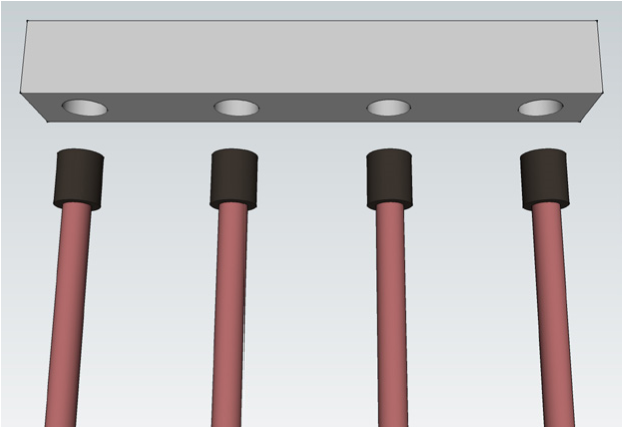
\includegraphics[height=4.5cm]{prefabricated-pile-cap1.png}
  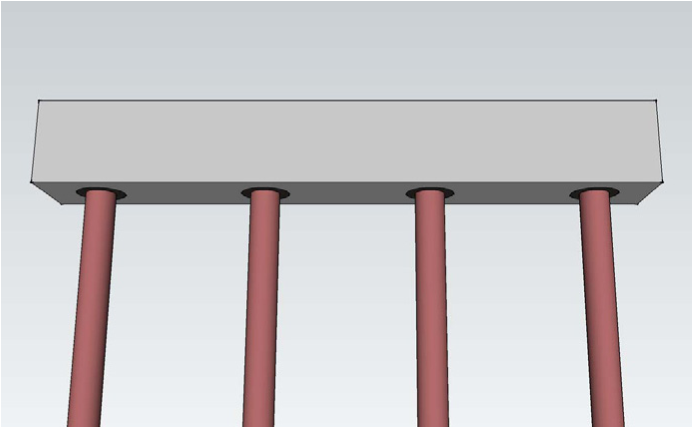
\includegraphics[height=4.5cm]{prefabricated-pile-cap2.png}
  % \caption{Prefabricated pile cap}
  \caption{预制桩帽}
  \label{fig:prefabricated-pile-cap}
\end{figure}

\emph{Design Considerations}. The material around the pile head is intended to have a very low elastic modulus to provide rotational capacity. Since the material for the detail experiences large strains, it must be able to accommodate these strains when subjected to the applied cyclic rotations.

Elastomeric material, regularly used as bearings for girder bridges, is recommended for the detail (Sherafati et al. 2013). Sufficient thickness needs to be provided to ensure the efficiency of the detail. Preliminary results indicate that the minimum thickness of elastomer should be 4 in.

\paragraph{Semi-Integral Pile Cap Design}
The pile cap in semi-integral bridges is mainly subjected to axial load and possibly the moment created by axial load eccentricity applied to the pile cap.
\paragraph{Seamless Details}
The design of the pile cap for a seamless bridge should follow the same procedure as for integral abutment bridges.

\subsubsection{End-Diaphragm (Backwall) Design}

In addition to being integral with the superstructure, the end diaphragm acts as a backwall for integral and semi-integral jointless bridge systems. As such, the end diaphragm is designed to resist forces resulting from soil loads and will henceforth be referred to as the backwall. The soil loads include the passive pressure force that is created by superstructure thermal expansion. The calculation of this passive pressure, Pp, is shown in Section 8.6.2.1.3.

Modeling, as shown in \cref{fig:lateral-pressure-superstructure} can be used to design the backwall.

\begin{figure}
  % \includegraphics[width=\linewidth]{graphic-file}
  \caption{Lateral pressure restraint by superstructure. (Oesterle et al. 2005)}
  \label{fig:lateral-pressure-superstructure}
\end{figure}

The following subsections discuss additional backwall design considerations that vary for each jointless bridge type.

\paragraph{Integral}

The backwall for an integral bridge abutment must be designed to adequately transfer forces across the construction joint and into the foundation cap for each direction in which the pile bends. This transfer of forces is illustrated through an example of strut-and-tie model in \cref{fig:lateral-pressure}. In this figure, Section AA shows the local section recommended for a local region ( d p + b ) over which the forces can be transferred and a suggested reinforcing pattern. The length d p is the distance from the forward face of the pile cap to the face of the pile.

\begin{figure}
  % \includegraphics[width=\linewidth]{graphic-file}
  \caption{Lateral pressure restraint by superstructure}
  \label{fig:lateral-pressure}
\end{figure}

\paragraph{Semi-Integral}

Semi integral backwalls do not require additional considerations above those outlined in Section 8.6.2.7.1. The one item of note, however, is that if removable forms are not used to form the bottom of the backwall over the foundation cap, the joint fill material used should be sufficiently stiff to support the concrete weight, yet flexible enough to not interfere with the movement permitted by the bearings. This has been successfully accomplished with expanded polystyrene filler.

\paragraph{Seamless}
The design of backwalls for seamless bridges should be the same as for integral bridges.


\subsubsection{Approach Slab Design}
Jointless bridges require approach slabs for two main reasons: 1) the slab needs to be positively attached to the
deck and/or substructure to eliminate the joint over the abutment, and 2) the slab must span the area behind the abutment where the potential for backfill settlement exists. Backfill settlement will occur and introduce voids
regardless of the degree of compaction and must be considered in design (Schaefer and Koch 1992)

\paragraph{Integral and Semi-Integral}

For both integral and semi-integral abutments, the length of the approach slab is determined by the extent of the
backfill. Gangarao and Thippeswamy (1996) determined that the rate of backfill settlement decreased significantly
beyond 20 ft. from the back face of the backwall. This is a typical standard approach slab dimension shown in several
state standards. The study by Schaefer and Koch (1992) demonstrated that backfill movements occur within a 1.5
horizontal to 1.0 vertical line from the bottom of the abutment for integral abutments. A general recommendation for
the design length of the approach slab is to conservatively set at a 2.0 horizontal to 1.0 vertical slope from the bottom
of the abutment. A 20 ft minimum should be considered for both integral and semi-integral abutments as shown in
\cref{fig:determination-approach-slab-length}.

\begin{figure}
  % \includegraphics[width=\linewidth]{graphic-file}
  \caption{Determination of approach slab length}
  \label{fig:determination-approach-slab-length}
\end{figure}

Additionally, experience from several states has found that the approach slab should be positively attached to the
backwall by at least No. 8 reinforcing bars anchored with a hook as shown in \cref{fig:determination-approach-slab-length}. The condition shown in the
figure allows for a separate pour of the approach slab designed as a simple span. Creating a moment connection
between the approach slab and the deck slab is not recommended. The connection should be detailed to act as a pin
with tension steel transferred across the approach span into the backwall for integral and semi-integral abutments. If a
moment connection is desired, it is recommended to use a seamless deck transition for the design (see Section
8.6.2.8.2).

A final consideration for the approach slab is the development of compression forces. Sufficient allowance for
expansion of the superstructure must be accommodated in the sleeper slab. (See Section 8.7.3 for sleeper slab details.)
Otherwise, compression can be introduced into the slab resulting from closing the expansion gap and then activating
the passive pressure behind the sleeper slab or contact with the adjacent roadway pavement, which is a major issue for
spalling and buckling of adjacent pavement.





\paragraph{Seamless Deck Transition Zone}
Details of seamless systems developed by SHRP 2 R19A are provided in Appendix E. The system is shown in \cref{fig:seamless-paving,fig:continuously-reinforced-jointed-pverment}.

Beyond the abutment a “Transition Zone” is required which replaces the approach slab. The proposed transition
introduces simplicity and ease of construction (Jung et al. 2007). The concept slowly transitions from a heavily
reinforced region to a plain jointed condition over an extended transition length. Within the heavily reinforced region,
crack spacing is quite small. As the level of reinforcement is reduced, the crack spacing increases. These cracks may
be allowed to occur naturally or may be forced by shallow saw cuts in the pavement.

Immediately adjacent to the bridge is a thickened and reinforced approach zone. The approach zone behaves
similar to a reinforced concrete slab bridge and is intended to carry flexural forces that may arise as a result of
settlement.

The design of the approach zone is similar to the design of an approach slab for an integral or semi-integral
bridge. The transition zone is not designed, per se, but the reinforcing spacing is reduced in specified stages. This
transition zone reinforcement is shown in \cref{fig:continuously-reinforced-jointed-pverment}.

\begin{figure}
  % \includegraphics[width=\linewidth]{graphic-file}
  \caption{Seamless paving over bridge transitioning to jointed pavement.}
  \label{fig:seamless-paving}
\end{figure}

\begin{figure}
  % \includegraphics[width=\linewidth]{graphic-file}
  \caption{Continuously reinforced to jointed pavement. (Jung et al. 2007)}
  \label{fig:continuously-reinforced-jointed-pverment}
\end{figure}

\subsubsection{Design of Superstructure-Pier Connection}
By definition, bridge decks in jointless bridges are continuous, including the region over the piers. The connection between the piers and the bridge deck could be integral, pinned, or expansion types, or be connected with a link slab. \cref{fig:bearing-jointless-bridges} shows these different configurations conceptually.

\begin{figure}
  % \includegraphics[width=\linewidth]{graphic-file}
  \caption{Integral, pinned, and expansion type bearings for jointless bridges}
  \label{fig:bearing-jointless-bridges}
\end{figure}

In integral type connections (Figure 8.27a), the pier and superstructure are monolithic with frame action developed between the superstructure and substructure. The advantage of this type of connection is the elimination of bearings. Further, the system provides higher levels of redundancy, especially in highly seismic areas. The longitudinal movement of the bridge superstructure is not affected by making the piers integral with superstructure. However, the longitudinal expansion of the deck must be considered in the design of the pier columns, pier foundations and their connection to the superstructure.

In pinned connections (Figure 8.27b), bearings are used to restrict longitudinal movement. Rotation at the bearing
is allowed. Although designated as a pin type connection, typical bridge terminology in which a bearing is not
permitted to move longitudinally is designated a fixed bearing, commonly denoted as “F” (Fixed) in traditional design
plans. For this connection, longitudinal movement between superstructure and pier is not permitted. Similar to
integral type connections, the longitudinal expansion of the deck must be considered in the design of the pier.

In expansion connections (Figure 8.27c), bearings are necessary and are required to accommodate both rotation
and longitudinal movements. This detail uses traditional expansion bearings as determined by design requirements.

For the three connection types shown in \cref{fig:bearing-jointless-bridges}, integral (a), pinned (b), and expansion (c), the superstructure
is made continuous over the pier. This can be accomplished in one of two ways: 
\begin{enumerate*}
  \item the superstructure splices can be positioned such that they are made at or near the dead load inflection points for the continuous bridge, or 
  \item a continuity splice can be used over the pier. This second option is commonly referred to as simple-for-dead-load, continuous-for-live-load. 
\end{enumerate*}
This construction method is shown conceptually in \cref{fig:sdcl-details} for an integral pier. The beams are placed as simply supported over the pier; the beams are either spliced mechanically or additional reinforcing is provided for the diaphragm; and finally, a closure pour is made.

\begin{figure}
  \begin{minipage}{0.32\linewidth}\centering
    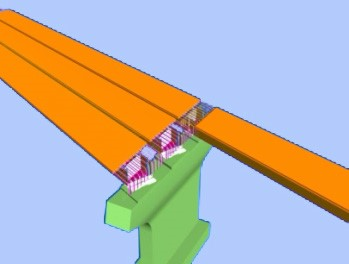
\includegraphics[height=3.5cm]{sdcl1.jpg}
    \subcaption{架设完成}
  \end{minipage}%
  \begin{minipage}{0.33\linewidth}\centering
    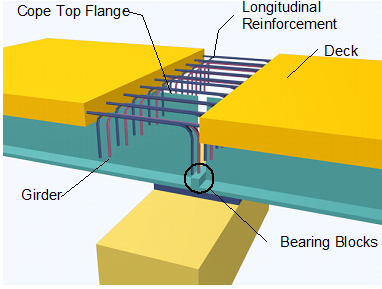
\includegraphics[height=3.5cm]{sdcl2.png}
    \subcaption{架设完成(细部)}
  \end{minipage}%
  \begin{minipage}{0.35\linewidth}\centering
    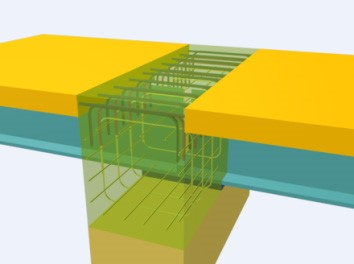
\includegraphics[height=3.5cm]{sdcl3.jpg}
    \subcaption{合龙段浇筑完成}
  \end{minipage}
  % \caption{Simple for dead and continuous for live pier detail after the placing of girders (a and b), and after the closure pour (c). (Azizinamini et al. 2008)}
  \caption{\acrlong*{sdcl}细部构造}
  \label{fig:sdcl-details}
\end{figure}

The last construction option is the expansion condition using a link slab (Figure 8.27d). A linkage slab is used
where the beams are not positively connected, as is the case with the other details shown in \cref{fig:bearing-jointless-bridges}. For this
condition, the superstructure is designed and constructed with traditional bearing considerations.

The design considerations for each of these pier cap connections are provided in the following sections.

\paragraph{Integral Pier Cap}

When making the superstructure truly integral with the pier cap, it must be recognized that both positive and
negative moments will be introduced to the cap from live loads and other transient loads. As such, sufficient strength
needs to be provided through the deck, integral diaphragm, and pier cap. While this type of connection eliminates the
need for bearings at the piers and can increase clearance, it introduces more complex forces in the superstructure and
the piers (see \cref{fig:integral-cap-completed}).

\begin{figure}
  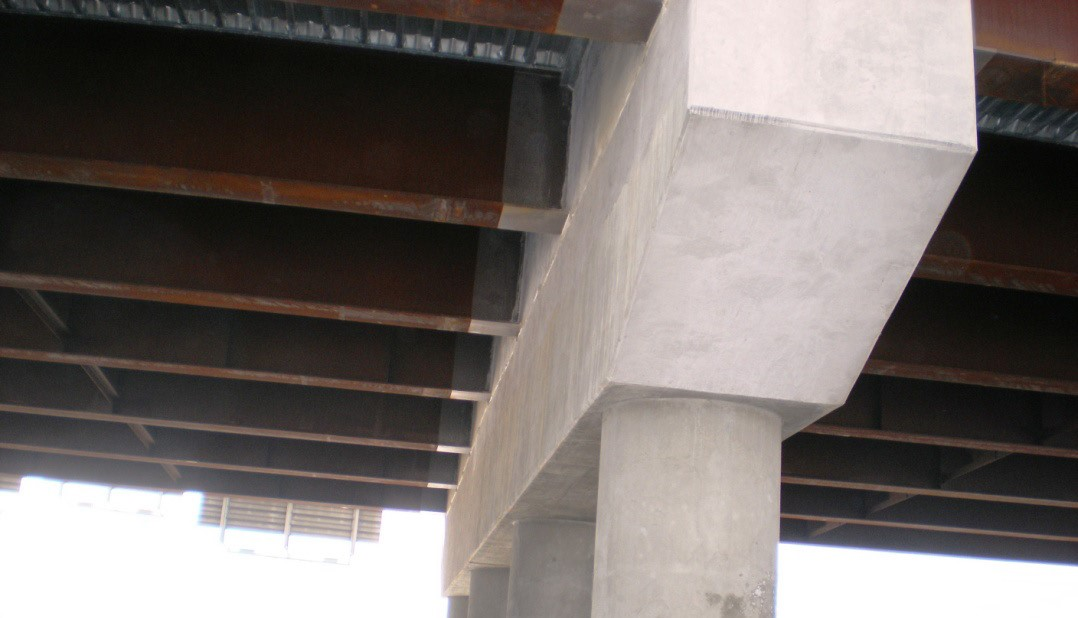
\includegraphics[width=0.7\linewidth]{integral-cap-completed.jpg}
  \caption{Integral cap as completed}
  \label{fig:integral-cap-completed}
\end{figure}

The longitudinal deflection movement of the foundation and the pier accommodates the total longitudinal movement expected at the top of the integral piers. (See Section 8.6.2.10 for additional information.) When designing the integral cap, the connection between the beams, continuity diaphragm, pier cap, and pier column must be sufficient to transfer the moments resulting from this deflection. Resolution of these forces should be computed by an analytical method or structural model with the ability to properly capture the behavior of the whole bridge system.

\paragraph{Fixed (Pinned) and Expansion Pier Caps}

Similar to the integral pier cap, the superstructure is made continuous over the pier for both fixed (pinned) and expansion pier caps. The difference is that it is not made integral with the pier caps. The connection between the superstructure and the pier is treated with traditional bearings.

Various details are used over the interior supports of multi-span bridges to eliminate joints. One of the concepts implemented by a number of owner agencies for concrete bridges has been the use of simple spans for dead load made continuous for live load (Freyermuth 1969; Oesterle et al. 1989) The girders are simply-supported for dead load, but continuity is achieved with deck steel as negative moment reinforcement over the piers. Also, the girders are made integral with the interior pier diaphragms and commonly positive moment reinforcement is included as shown in \cref{fig:continuity-live-load-connection}.

\begin{figure}
  % \includegraphics[width=\linewidth]{graphic-file}
  \caption{Precast, prestressed girders connected with live load continuity.}
  \label{fig:continuity-live-load-connection}
\end{figure}

Badie et al. (2001) discussed the alternate use of an interior steel pier diaphragm with prestressed girders to speed
construction and achieve better overall design economy. The concept of a simple span made continuous has also been applied to eliminate interior joints and improve the construction speed and design economy for short- and medium-
span steel girder bridges (Azizinamini et al. 2008).

As discussed in Section 8.6.2.4, attention must be paid to the effects of providing positive moment restraint at the
diaphragms. Some simple-made continuous prestressed concrete girder bridges have experienced severe cracking in
the girders near the interior diaphragms. One example that has been studied extensively was on the Francis Case
Memorial Bridge spanning the Washington Channel of the Potomac River in the District of Columbia (Telang and
Mehrabi 2003). The prime cause of this distress was the restraint of upward camber of the prestressed girders under
the influence of prestressing and temperature gradient. According to Telang and Mehrabi (2003), “By providing a
large amount of positive moment reinforcement at the diaphragms, designers inadvertently make the diaphragm area
stronger than the adjacent girder sections, thereby forcing the cracking to occur in far more critical but weaker areas
of the girder span.” The article states, “In closing, it is important to note that this seemingly simple transformation of
simple-span prestressed girders to continuous spans should be attempted with caution, and significant attention must
be paid during analysis and design to include loading conditions that can cause counterintuitive behavior such as
secondary positive moments at the piers. Most importantly, positive moment reinforcement should be designed and
detailed such that any cracking, if it occurs, should be limited to the relatively less critical diaphragm region of this
type of structural system.” Further discussion of this problem and solutions to avoid it have been published by
Oesterle et al. (2004a) and Arockiasamy and Sivakumar (2005) and are discussed in Section 8.6.2.4.

\paragraph{Link Slab Expansion Pier Cap}
A link slab is a type of detail used in conjunction with existing or new bridges having girders that act as simple
beams for both dead and live loads. In this type of deck detail, the slab spans continuously over the longitudinal gap
between the adjacent span girders while the girders are kept as simple-spans. The length of the deck connecting the
two adjacent simple-span girders is called a link slab (Caner and Zia 1998). Link slabs generally require less deck reinforcement, but have more girder positive moment demands than simple-made-continuous designs. Limited
analysis and laboratory experiments were carried out and design recommendations are provided in Caner and Zia
1998. The use of this detail has been very limited due to field observed cracking. In fact, link slabs are not common in
snow belt states. A crack is invariably formed due to deck slab rotation as the bridge is loaded with live loads.

\begin{figure}
  % \includegraphics[width=\linewidth]{graphic-file}
  \caption{Conceptual detail for link slab.}
  \label{fig:conceptual-detail-link-slab}
\end{figure}

SHRP 2 R19A research studies on the link slab indicated that it offered negligible rotational end restraint to the
bridge girders and that the link slab can be analyzed as a beam subjected to the same end rotations as the adjacent
girders. The researchers found that under service-load conditions, the link slab would crack primarily due to bending.
In addition, prior research by Gastal (1989) and El-Safty (1994) were capable of predicting the forces, stresses and
crack widths in the link slab due to thermal and creep and shrinkage effects. Caner (1996) modified the procedures
developed by Gastal and El-Safty to properly capture the link-slab actions. All of these solutions were based on beam
theory. The reinforcing bar stresses compared reasonably well with the data measured from the experimental tests.
The predicted crack widths were somewhat larger than the measured crack widths. The researchers concluded that
bending and cracking under live load plus impact are the governing factors that must be considered in the design of
the link slab.

Caner and Zia (1998) suggested design of the link slab using only one layer of rebar placed near the top of the
deck, but suggested that two layers could be used to improve performance in bridges having horizontal restraints.

\subsubsection{Design of Integral Piers}
As previously discussed in the section on design of integral pier caps the total longitudinal movement expected at the top of integral piers is accommodated by two modes of deformation: longitudinal movement via rotation of the foundation system and flexural deflection of the pier. Pier deflection can be both elastic and inelastic in response.

\paragraph{Foundation Rotation}
For spread footings, Zederbaum (1969) provides an equation to estimate the rotational stiffness of the soil or rock responding to an applied moment:
\begin{equation}
  K_\theta=\frac{3E_\text{s}I_\text{f}}{b}
\end{equation}
\begin{EqDesc}{K_\theta}
  \item[K_\theta] 基础的转动刚度;
  \item[b] 承台扩散宽度的$1/3$;
  \item[E_\text{s}] 土体或岩石的压缩模量;
  \item[I_\text{f}] 承台基础的抗弯惯性矩。
\end{EqDesc}

For pile-supported and drilled shaft-supported foundations, the rotational stiffness is estimated from the elastic stiffness of the pile or shaft group. Rotation of the foundation can be attributed to the elastic shortening and elongation of the piles or shafts for multiple rows. Note that the elongation and shortening add additional uplift and downward forces, respectively, that must be accounted for in the foundation design. In a single row of piles or drilled shafts, the rotational stiffness is based on the cantilever response of the single row. The length of the cantilever is based on the soil-structure interaction at the foundation and can be based on the assumed or calculated point of fixity for the pile or shaft.

\paragraph{Pier Displacement}
The differential between the pier displacement at the integral cap and the rotation of the foundation is the deflection of the pier column. The resulting design moment can be estimated by the following. First, the expected movement of the superstructure at the pier cap should be calculated, as outlined in Section 8.6.2.3. Alternately, this can be sufficiently approximated by determining the point of zero movement on the bridge and multiplying the end displacement by the ratio of the distance from the fixed point to the pier to the distance from fixity to the end support. Second, assume that 30\% of the expected lateral deflection is accommodated by the foundation rotation. Thirty percent is based on a parametric study that demonstrated foundation rotation can vary from 30\% to 80\% with an average close to 45\%. Third, the anticipated bending moment should be calculated using the equation:

\begin{equation}
  \label{eq:moment-cap}
  M = \frac{6EI_\text{c}\Delta b}{H^2}
\end{equation}
\begin{EqDesc}{\Delta b}
  \item[E] concrete modulus
  \item[I_\text{c}] effective section modulus
  \item[\Delta b] lateral deflection at pier cap
  \item[H] height of the pier
\end{EqDesc}

Note that the value of the effective section modulus may depend on the applied loading and thus a simultaneous or iterative solution may be required. For fixed (pinned) continuous piers, divide the result of \cref{{eq:moment-cap}} by 2 (fixed end moment for a fixed-guided beam is one half that of a fixed-fixed beam). The value of the effective section modulus for reinforced concrete piers can be obtained from \cref{eq:effective-section-modulus}.
\begin{equation}
  \label{eq:effective-section-modulus}
  I_\text{e} = \left(\frac{M_\text{cr}}{M_\text{a}}\right)^3 I_\text{g} + \left[ 1-\left(\frac{M_\text{cr}}{M_\text{a}}\right)^3\right] I_\text{cr}
\end{equation}
\begin{EqDesc}{M_\text{cr}}
  \item[M_\text{cr}] 开裂弯矩;
  \item[M_\text{a}] 作用弯矩;
  \item[I_\text{g}] 毛截面惯性矩;
  \item[I_\text{cr}] 截面开裂弯矩。
\end{EqDesc}

\subsubsection{Design of Wingwalls}
The design of wingwalls depends on their orientation relative to the abutment stem, their method of support, and the abutment skew. There are various possible configurations for wingwalls, but the traditional configurations include U-shaped, straight, or flared, the latter being some degree of angle between the other two.

Oesterle et al. (2005) indicates that the U-shape configuration is preferable for wingwalls in that this configuration inherently reduces the passive pressure introduced by the longitudinal movement of the abutment end diaphragms. Additionally, they note that the U-shape configuration conveniently contains the soil behind the abutment and decreases bulging of the embankment soil.

Use of both straight and flared walls leads to the development of passive pressure on the wingwalls as the jointless abutment moves. Oesterle et al. (2005) note that this pressure can be expected to decrease as the distance from the abutment increases, but that the degradation cannot be effectively predicted. Thus, the wingwalls need to be designed for the same passive pressure as that of the abutment end diaphragm across the length.

For integral and seamless bridges, additional considerations for wingwalls include the loading effect they have on the bridge structure. When cantilevered from the abutment stem, the weight of the wingwalls will create additional torsion and/or bending along the length of the abutment. These forces are resisted by a counteracting negative moment at the end of the external beam or girder.

If wingwalls for integral abutments are placed on supports, such as piles or spread foundation, the support must be able to accommodate the movements of the jointless bridge as well. For this condition, Oesterle et al. (2005) note that the shear and moment developed in the wingwall foundation must be transferred through the wingwall structure to the abutment and superstructure. They also note that U-shaped wingwalls on piles create significant resistance to abutment rotation, which creates partial fixity for beam end moments on the exterior beams or girders. These additional moments need to be included in the design of the connections of the exterior beams to the integral abutment.

\section{Details}
The introduction of different mechanisms for transferring force to the foundations requires that additional details
be considered when designing jointless bridges. The following section presents specific details for each jointless
bridge type. In this section, the term backwall is used to describe the end diaphragm that resists soil loads.

\subsection{General Abutment Details for Jointless Bridges}
In this section, details that have been used successfully in the past by some states are presented along with general
concepts. The figures presented represent recent research efforts and the accumulated experience of several states that
have used jointless bridge technology.

\subsubsection{Integral Abutments}
\label{subsubsec:integral-abutments}
\cref{fig:general-integral-abutment-concept} shows the overall concept for an integral bridge abutment including the typical layout with the beam,
end diaphragm (backwall) and pile cap, all integral. Although it is not necessary in all cases, the beam shown in this
figure is sitting on a temporary pedestal to achieve proper alignment before being cast integral with the rest of the
abutment. Alternatively, the cap can be stepped to accommodate elevations prior to pouring the backwall. For proper alignment and to allow for rotations that occur when placing the beam, a small elastomeric pad should be placed at the
girder bearing even though each beam will eventually be cast composite with the abutment. Note that the need to
design the pads and for what capacity has not been thoroughly studied. The pads need not be designed to meet the
criteria for rotational capacity, which is now addressed as a shear strain component. The maximum rotation of the
pad is realized during placement of the beam. A reasonable assumption is to design the pad to accommodate only
non-composite bearing pressure.

\begin{figure}
  % \includegraphics[width=\linewidth]{graphic-file}
  \caption{General integral abutment concept}
  \label{fig:general-integral-abutment-concept}
\end{figure}

Drainage is also important to avoid ice expansion and removal of the backfill by washout. A drain pipe should be
placed at the appropriate location to properly remove any water that might otherwise accumulate behind the backwall.

Additional end diaphragm details are presented in \cref{fig:integral-abutment-details}. Note that an H-pile foundation is shown in the
figure; however, each of the foundation types noted in the strategy table in Section 8.5 can be interchanged. The
minimum embedment length of 2 ft., within pile cap, should be maintained for H-piles, prestressed piles, and CFT
piles, as shown in Figure 8.34. Also shown in the figure is an approximate cap height of 5 ft, typical of the cold
weather regions, which allows for embedment below the frost depth and to provide 2 ft between the finished grade
and the bottom of the beam. A depth of 3 ft to 3.5 ft is more common where frost depth need not be considered.
Another alternative to the holes through the beam shown in the figure is to use threaded inserts, which are preferred
by some precast concrete companies to ease securing them in the forms.

\begin{figure}
  % \includegraphics[width=\linewidth]{graphic-file}
  \caption{Integral abutment details.}
  \label{fig:integral-abutment-details}
\end{figure}

\cref{fig:integral-abutment-rotation-detail} is an adaptation from an Ohio DOT standard drawing showing a prestressed concrete beam. Now a
standard detail for most prestressed girders includes providing holes through the beam for reinforcing.
 This
reinforcing provides continuity though the backwall for bending and limits the differential deflection between the
superstructure and backwall where tension forces develop in the top portion of the web.

In contrast to the design recommendations in Section 8.6.2.7, the state of Ohio allows for rotation in the backwall
across the construction joint instead of designing rebar to transfer the forces through the stem. The configuration is
used to accommodate the rotation of the superstructure as shown in \cref{fig:integral-abutment-rotation-detail}. At the centerline of bearing,
reinforcing is crossed at the bearing pivot location, and expansion joint material is placed so as to permit a limited
amount of rotation.
 Note that Ohio limits the length of their bridges with integral abutments to 250 ft, so
consideration of this limit should be made before adopting this detail for other bridges.

\begin{figure}
  % \includegraphics[width=\linewidth]{graphic-file}
  \caption{ Integral abutment rotation detail.}
  \label{fig:integral-abutment-rotation-detail}
\end{figure}

\cref{fig:integral-abutment-details2} presents another standard integral detail drawing from the New York State Throughway Authority,
which shows a steel beam connection. This detail is more typical of DOT design standards in that the reinforcing is
continuous across the construction joint. Additionally, when comparing this detail with \cref{fig:integral-abutment-details}, although both
details have had repeated success, there are two obvious differences: 
\begin{enumerate*}
  \item \cref{fig:integral-abutment-details} shows a bent hook bar connecting the approach slab, whereas \cref{fig:integral-abutment-details2} shows that continuity is maintained by a straight bar connecting the approach slab to the deck; and 
  \item the \cref{fig:integral-abutment-details} detail utilizes a shear key, while the \cref{fig:integral-abutment-details2} detail relies solely on the continuity of the reinforcing across the construction joint. Each detail has demonstrated success in application and the designer should consider which option may be more appropriate for each bridge’s unique situation.
\end{enumerate*}

For more information on backwall detailing see Section 8.7.2.

\begin{figure}
  % \includegraphics[width=\linewidth]{graphic-file}
  \caption{Integral abutment details. (New York DOT)}
  \label{fig:integral-abutment-details2}
\end{figure}

\subsubsection{Semi-Integral Abutments}
\cref{fig:semi-integral-abutment-concept} shows the overall concept for a semi-integral bridge abutment. It includes the typical layout with the beam and end diaphragm (backwall) cast integral.

\begin{figure}
  % \includegraphics[width=\linewidth]{graphic-file}
  \caption{General semi-integral abutment concept.}
  \label{fig:semi-integral-abutment-concept}
\end{figure}

Drainage and porous backfill are necessary for the same reasons as for integral abutments—formation of ice and integrity of the backfill. In semi-integral abutments, two bearing strategies have been used successfully: 
\begin{enumerate*}
  \item the pile cap may be cast level and the superstructure superelevation can be accommodated through the use of bearing pedestals, and 
  \item the second method is to step the pile cap. In this case, the polystyrene filler must be used on both the top of the cap and on the sides of the step to allow for movement. 
\end{enumerate*}
Due to the nature of the superstructure movement it is recommended that the first case with pedestals be used for locations of high skew (larger than 20°) and bridges on a curve. If it is desired to inspect the bearings during the life of the bridge, removable filler material should be placed in front of the bearings.

\cref{fig:semi-integral-details} shows the successful detailing strategies that have been used in various states. The foundation shown is for a drilled shaft, but other foundation types are equally applicable. Similar to integral abutments, dowel holes are placed through the beam or girder. Unlike integral abutments, bearings are used to accommodate movement between the superstructure and the foundation. Efforts must be made to seal the gap between the cap and backwall yet still accommodate movement. This seal has traditionally been a preformed filler surrounding the bearing area and a layer of waterproofing applied to the rear face of the seam prior to placing the backfill. For more information on backwall detailing see Section 8.7.2.

Other than the backwall and treatment of the bearing area, detailing for the rest of a semi-integral abutment is the same as traditional design.

\begin{figure}
  % \includegraphics[width=\linewidth]{graphic-file}
  \caption{Semi-integral details}
  \label{fig:semi-integral-details}
\end{figure}

\cref{fig:semi-integral-details-extended-diaphragm} shows an alternate detail used in instances in which the diaphragm is extended and a lip is dropped
down over the pile cap. This detail replaces the neoprene sheeting that provided the barrier between the porous
backfill and the expanded polystyrene filler surrounding the bearings. Preformed elastomeric material is placed
between the extended diaphragm and the abutment stem.

\begin{figure}
  % \includegraphics[width=\linewidth]{graphic-file}
  \caption{Semi-integral details with extended diaphragm.}
  \label{fig:semi-integral-details-extended-diaphragm}
\end{figure}



\subsubsection{Seamless Abutments}
Detail recommendations for the transition zone are not well established and thus no standard details are available for reference. However, the recommendations for the abutment cap and backwall are the same as those presented in \cref{subsubsec:integral-abutments}.

\subsection{Pile Cap and Backwall}
Oesterle et al. (2005) recommend that vertical reinforcement for the moment from the soil load be distributed
with 75\% of the bars within 25\% of the beam spacing on either side of the beam. Furthermore, for crack control they
recommend the center-to-center spacing of the flexural reinforcement not exceed (in inches):
\begin{align}
  s &\leqslant \frac{540}{f_\text{s}}-2.5c_\text{c} \quad \text{或}\\
  s &\leqslant 12 \left(\frac{36}{f_\text{s}}\right)
\end{align}
\begin{EqDesc}{f_\text{s}}
  \item[c_\text{c}] clear cover from the nearest surface in tension
  \item[f_\text{s}] calculated stress (ksi) at service load, or alternately as $0.60Fy$
\end{EqDesc}

This limitation is taken from ACI 318-05 Section 10.6.4 rules for the distribution of flexural reinforcing to control cracking in one-way slabs. Further commentary on this requirement can be found in that section.

\subsection{Sleeper Slab}
A sleeper slab is appropriate for all integral or semi-integral bridges and is placed at the roadway end of the
approach slab. The intent of this slab is to provide a relatively solid foundation for the far end of the approach slab
and to provide a location for limited expansion and contraction (see \cref{fig:sleeper-slab-detail}). Although no formal design is
suggested, a typical suggested detail has been provided by Wasserman and Walker (1996).

\begin{figure}
  % \includegraphics[width=\linewidth]{graphic-file}
  \caption{Suggested helper (sleeper) slab details. (Wasserman and Walker 1996)}
  \label{fig:sleeper-slab-detail}
\end{figure}

A potential problem with \cref{fig:sleeper-slab-detail} is that it presents a potential for cracking in the approach pavement where it
suddenly transitions to the thin piece above the sleeper slab. Whereas this might ease final grading, it is preferable to
have the stem of the inverted “T” of the sleeper slab extend to final grade and thus avoid any sharp transitions.

The state of New York has adopted this sleeper slab detail and modified it to marry the adjoining pavement design
based on the type of surfacing used. \cref{fig:slab-concrete-pavement,fig:slab-asphalt-pavement} show the sleeper slab for concrete and asphaltic
pavements respectively. In these figures, note how the state formed the joint such that both the pavement and
approach slab are both graded at full depth up to the sleeper slab that provides the transition.

\begin{figure}
  % \includegraphics[width=\linewidth]{graphic-file}
  \caption{Sleeper slab with concrete pavement approach. (New York DOT)}
  \label{fig:slab-concrete-pavement}
\end{figure}
\begin{figure}
  % \includegraphics[width=\linewidth]{graphic-file}
  \caption{Sleeper slab with asphalt pavement approach. (New York DOT)}
  \label{fig:slab-asphalt-pavement}
\end{figure}

The location of the sleeper slab should be placed so that the entirety of the slab is outside the failure plane as discussed in Section 8.6.2.8.1.

\subsection{Details for Skewed and Curved Bridges}
Transverse movements of integral abutments associated with large skews or horizontal curves should be accommodated by the details for barrier walls, drainage structures, and the ends of the approach slabs. In addition, the foundation and pier structure stiffness will likely be significant for movement parallel to the pier cap. Therefore, it is recommended that the connection between the bottoms of the girders and diaphragms and the pier caps be flexible in this direction. This approach, however, may not be appropriate for seismic design, in which case the design of the diaphragms should consider the interior pier restraint of the rigid body rotations that result from passive abutment restraint of longitudinal thermal expansion.


\section{Construction}
\subsection{Construction Stability}
Due to concerns about the repetitive bending stresses on the pile, it is recommended that no seam (weld) be
placed at the top 30 ft of the pile. This will ensure proper ductility and eliminate the possibility of having a poor
fatigue detail near the region of higher bending response. Additionally, this will better ensure proper alignment of the
pile at the cap.

The order of construction is also important as described in \cref{subsec:construction-sequencing}.

\subsection{Utilities}
Non-flexible utilities should not be permitted to pass through integral and semi-integral abutments. Multiple
DOTs report experiencing problems in which the flexibility of the integral cap creates issues with rigid utilities. Only
utilities that are able to sufficiently flex with the movement of the integral abutment should be permitted, but it is
preferable to locate all utilities adjacent to the bridge structure.

\subsection{Cracking Control}
Vertical cracks have often been found at the bottom of diaphragms between precast beams over the piers, in the
positive moment connection region near the external (fascia) girders.
 On the interior girders encased in the
diaphragm, spalling of the diaphragm has been observed near the bottom flange. This spalling resulted from the
bottom flange slipping outward (away from the diaphragm) due to the end rotation of the girder associated with creep
and thermal changes. These vertical cracks in the diaphragm and end rotation of the girders serve to relieve tensile
stresses due to creep, shrinkage, and thermal movement and are not detrimental to the integrity of the structure.
Attempts to control this cracking through over-reinforcing may result in cracks in less desirable locations.

Horizontal cracks and efflorescence have been found on the forward face of integral abutments at the construction
joint on top of the pile cap. This can be alleviated by placing adequate sealing from water behind the stem across the
construction joint.

Settlement of the approach slab is common and this can cause cracking and further damage to the barrier rail.
Rails that are attached to both the deck and approach slab should be jointed to accommodate the differential
settlement.

\subsection{Construction Sequencing}
\label{subsec:construction-sequencing}
Guidelines for concrete bridge deck materials and construction to control transverse cracking in concrete bridge
decks are presented in NCHRP Report 380 (Krauss 1996). Among the issues that affect deck cracking are weather,
time of placement, curing, vibration, finishing, loads, and placement sequencing. Certain current practices are
presented here for jointless bridges.

For jointless bridges the construction sequence should generally be as follows:
\begin{enumerate}
  \item Embankment should be completed prior to pile driving and allow for consolidation (if required).
  \item Piling should be placed and pre-drill holes filled and forms constructed (if used).
  \item Abutments and wingwalls should be constructed to the elevation of bearing seat.
  \item Semi-integral elastomeric bearings should be set; or for integral beam pads should be set allowing for
rotation from beam and deck dead load.
  \item Beams should be set.
  \item The deck slab and the integral backwall should be cast. The ends of the slab should be poured last in
order to minimize locked-in stresses at the supports.
  \item Drainage and backfill should be placed behind the abutments after the deck has achieved the appropriate
strength. It is important that the backfill be placed simultaneously behind each abutment so the bridge is
not inadvertently shifted in the unsupported direction.
  \item The approach slab should be cast, ideally with the bridge in the thermally contracted position (i.e., early
morning). This avoids putting the slab into tension until the concrete has gained sufficient strength.
\end{enumerate}

It should be emphasized that simultaneous placement of the abutment backfill (7) is particularly important for
semi-integral abutments. The reason for this emphasis for semi-integal bridges is that the superstructure sits on
flexible bearings rather than being positively attached to the abutment, and is more likely to move due to the pressure
from the compacting procedures.

\subsection{Fill Compaction}
Construction can follow normal compaction procedures as specified by the owner agency except as noted in the
construction sequencing. Fill compaction has been modified and adjusted using several variables, including the use of
specialized material. However, general experience has indicated that properly compacted normal fill material is
sufficient for jointless bridge construction, and proper drainage behind the backwall is more important.



\section{Maintenance and Repair}
\subsection{Problems with Jointless Construction}
Although adoption of integral-type bridges will eliminate some of the more troublesome problems associated with
jointed bridges and yield significantly more durable structures, they will not eliminate endemic highway construction
problems that are somewhat related to accelerated construction, all-weather construction, marginal construction
supervision, and other construction issues identified in \cref{chp:materials} on materials and \cref{chp:bridge-decks} on bridge deck.

Transverse and diagonal deck slab cracks, stage construction issues, lateral rotation of superstructure, erosion of embankments, marginal quality of structure movement systems, and other problems have appeared to trouble design, construction, and maintenance engineers. Except for early-age deck slab cracking, these problems are generally the result of failure to anticipate and apply typical design and construction provisions to achieve trouble-free construction and more durable structures.

\subsection{Deck Cracking}
Diagonal deck slab cracks located at acute corners of integral-type bridges are occasionally reported. When
constructing integral-type bridges, stationary abutments and moving superstructure must be joined together by cast-in-
place continuity connections. Consequently, these connections could be stressed and cracked if a substantial
temperature drop were to occur during initial concrete setting, or if concrete placement sequences were not suitably
controlled. To address this problem, one or more of the following procedures should be used: place continuity connections at sunrise, place deck slab and continuity connections at sunrise, place continuity connections after deck
slab placement, or use crack sealers.

\subsection{Lateral Rotation of Semi-Integral Bridges}
One of the primary aspects of semi-integral bridges that must be considered and addressed is the design and
proper orientation of guided bearings for the superstructure of skewed bridges. Unfortunately, many of the retention
devices currently being used are not fully functional because of friction and binding and consequently, the long-term
stability of some abutments, especially those not supported by rigid foundations, may not have been provided for
effectively. However, it appears inevitable that this aspect of the semi-integral bridge concept will be improved when
bearing manufacturers and bridge design engineers combine their expertise to design and manufacture more
functional structure movement systems for these applications.

\subsection{Approach Slabs}
Shortly after the state of Ohio adapted the integral concept to continuous steel beam bridges in the early 1960s,
slab distress was experienced. Where the bridges in question were constructed adjacent to compressible asphalt
concrete approach pavements, approach slab seats at the ends of bridge superstructure were found to be fractured,
approach slabs had settled, and the vertical discontinuity in the roadway surface at the approach slab/superstructure
interface was hindering movement of vehicular traffic.

\subsection{Drainage}
Washout has been noted on several existing structures in which drainage was not properly designed or
maintained, including some where the piles became exposed. It is imperative that proper drainage material including
geotextiles and perforated piping be placed behind the abutments. The preferred alternative is to direct water away
from the bridge approach, but it is acknowledged that this can be difficult to accomplish in many cases.

Additionally, improper drainage can lead to washout at one end of the bridge and not the other. For semi-integral
abutments, this leads to an unbalanced soil pressure, which can lead to additional maintenance issues at the bearing
locations.

Drainage can also affect settlement of the sleeper slab and create settlement of the approach slab. It is
recommended that runoff be intercepted or diverted so that it does not reach the end of the approach slab.

In regions that experience freezing temperatures, proper drainage is also important to minimize the potential for
frozen soil behind the abutment. The magnitude of the potential restraining force is unknown for frozen soil, but it
will be minimized with proper drainage (Briaud et al. 1997).

\subsection{Cycle-control Joints}
Probably the most significant unresolved problem regarding integral and semi-integral bridges is the availability
of cost-effective functional and durable cycle-control joints, which are the moveable transverse joints used between
approach slabs of integral-type bridges and approach pavements. The usual pavement movement joints, composed of
preformed fillers, are currently being used for the shortest bridges. For the longest bridges, finger-plate joints with
easily maintainable curb inlets and drainage troughs have been successfully employed. However, for intermediate-
length bridges, development of a suitable cycle-control joint is still in the evolutionary stages.

\subsection{Deck Replacement}
\cref{fig:flanges-buckled} shows what can happen when the proper procedures and sequences for deck replacement and integral
abutment backfilling are not followed. It should be anticipated that large compressive forces are acting on the whole
structure as a result of soil pressure on the abutments and restrained expansion of the girders. In order to ensure the
global stability of the structure, one of two procedures must be followed. The first procedure, which should always be
used for whole deck replacement, is to use proper construction sequencing as follows:
\begin{enumerate}
  \item Remove the approach slab.
  \item Remove backfill to the bottom of the stem for integral or to the bottom of the end diaphragm for semi-
integral abutments. Excavation should be done simultaneously behind both backwalls.
  \item Remove the deck.
  \item Replace the deck according to the guidance provided in Section 8.8.4.
\end{enumerate}

The second option is to calculate the stress applied by the passive pressure of the abutment backwalls. This force
can then be applied to the superstructure with portions of the deck removed to check the stability of the system and
each structural item that might be affected by the removal of the deck. This includes checking both local and global
buckling stability. It is recommended that this be used only for partial width deck repair.

\begin{figure}
  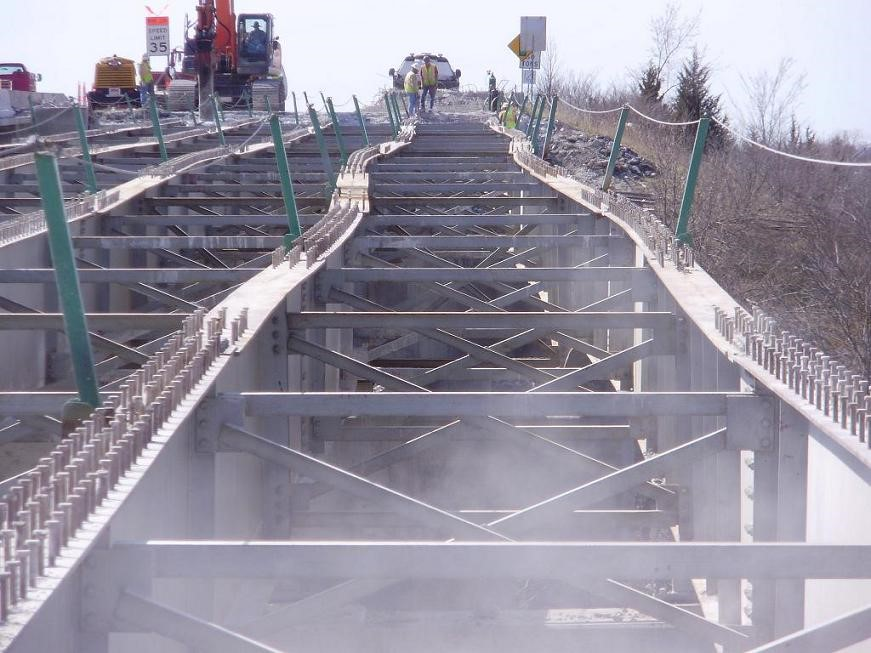
\includegraphics[width=0.6\linewidth]{flanges-buckled.jpg}
  \caption{Buckled girder flanges due to improper deck sequencing.}
  \label{fig:flanges-buckled}
\end{figure}

\subsection{Bearing Replacement for Semi-Integral}
An additional factor when detailing semi-integral jointless bridges, should bearing repair or replacement be
required, is to incorporate appropriate features at the initial design stage to facilitate superstructure jacking. In general,
since superstructure and abutments in semi-integral bridges are separated by elastomeric bearings, it would be easy to
place flat jacks between the abutment and the end diaphragm to raise the superstructure and approach slab and allow
replacement of the bearing.

\section{Retrofits}
A large percentage of existing bridges are simple span bridges that rely on expansion joints at piers and abutments
to accommodate longitudinal movements. Most of the deficient bridges in the United States include these jointed
structures, which require upgrade and repair. Retrofitting existing jointed bridges to jointless ones is highly
recommended.

The following considerations are required in integral conversion (Leathers 1990):
\begin{enumerate}
  \item The existing structural elements should be able to properly function without the expansion joint.
  \item Movement calculation should be based on the LRFD Specifications.
  \item Continuity can be achieved by making either the deck or the girders continuous.
  \item All obsolete and/or deteriorated bearings should be replaced with elastomeric bearing devices.
  \item If the abutment is unrestrained, a fixed integral condition can be developed for many of the shorter bridges. Abutments that are free to rotate are considered unrestrained, such as a stub abutment on one row of piles or an abutment hinged at the footing. A semi-integral condition can be developed for restrained abutments.
\end{enumerate}

\subsection{Details over the Pier}
Two practical options that can be used with or without integral abutments are available for retrofitting existing
jointed bridges into jointless bridges.

\begin{enumerate}
  \item Provide beam continuity for live load only. In this case, the negative moment continuity is provided over the piers, with or without positive moment continuity at these locations.
  \item Only provide deck slab continuity. In this option, although the deck is continuous, beams are technically, simply supported. This method involves removing some length of slab at the ends of the adjacent beams, splicing the existing reinforcement and adding new bars, then recasting that part of the deck.
\end{enumerate}

\paragraph*{Link Slab}
When retrofit of an existing open joint is considered, the following approach may be used as shown in \cref{fig:integral-conversion-piers} (Note for this detail only the deck is made continuous.)
\begin{enumerate}
  \item Remove concrete as necessary to eliminate existing armoring.
  \item Add negative moment steel at the level of existing top-deck steel sufficient to resist transverse cracking.
  \item Reconstruct with regular concrete to original grade.
\end{enumerate}

\begin{figure}
  % \includegraphics[width=\linewidth]{graphic-file}
  \caption{Integral conversion at piers. (Leathers 1990)}
  \label{fig:integral-conversion-piers}
\end{figure}

Since the deck slab would be exposed to longitudinal flexure due to rotation of beam ends responding to the movement of vehicular traffic, cracks will occur over the link slab. However, for short and medium span bridges, the deck cracking associated with such behavior is preferred over long-term consequences associated with open moveable deck joints or poorly executed joint seals.

\subsection{Details over the Abutment}
For existing stub abutments with a single row of piles, the following procedure shown in \cref{fig:conversion-moveable-integral} should be used (integral abutment retrofit).
\begin{enumerate}
  \item Check the capacity of piles and pile-cap connection for the expected movement.
  \item Remove the approach slab, and excavate backfill to the elevation of existing ground on front face.
  \item Demolish the existing backwall to top of bridge seat. Cast reinforced concrete around beam ends.
  \item Then provide drainage, backfill, and new approach slab behind the new abutment.
\end{enumerate}

\begin{figure}
  % \includegraphics[width=\linewidth]{graphic-file}
  \caption{Conversion of a bridge with moveable deck joints at the superstructure-abutment interface with integral abutment (a) before conversion, and (b) after conversion.}
  \label{fig:conversion-moveable-integral}
\end{figure}

For existing stub abutments with rigid foundation or existing full height wall abutments, the following procedure should be used (semi-integral abutment retrofit).
\begin{enumerate}
  \item Remove the approach slab and excavate the backfill to the elevation of existing ground on front face.
  \item Remove the existing abutment backwall to the top of bridge seat.
  \item Provide a sliding surface between the pile cap and the abutment stem which is cast integrally with the
  beam ends and approach slab.
  \item Provide details for both horizontal and vertical sliding joints using lateral guide bearings, sheet seals, and
  drainage and backfill.
\end{enumerate}

\begin{figure}
  % \includegraphics[width=\linewidth]{graphic-file}
  \caption{Conversion of a very short span bridge with moveable deck joints at the superstructure-abutment
  interface with integral abutment (a) before conversion, and (b) after conversion.}
  \label{fig:conversion-moveable-integral-short-span}
\end{figure}

\subsection{Converting Jointed Bridges to Jointless Bridges}
General experience has shown that most common bridge types can be converted to jointless bridges to enhance their performance with the same goal as new construction (i.e., joint elimination). Examples of candidates that have already been converted are pin-and-hanger bridges and multi-span, simple span bridges for both steel and concrete superstructures.

Several states have had success converting old pin-and-hanger expansion joints to a bolted full moment connection, thus eliminating the expansion joints.

The state of New Mexico has presented several case studies (Maberry et al. 2005). In one project, they converted simple span concrete girders by incorporating a link slab. The project demonstrated that attention must be paid to the bearings. The greatly increased expansion that would transfer to the outer bearing locations was overlooked by the retrofit assessment. Subsequently, the resulting expansion loads were absorbed by the pile caps, which quickly deteriorated.

The key to any conversion is the ability of the bridge to withstand the new continuity loading and expansion demands introduced by the changed load path. Due to the complex nature of the converted structure, it is recommended that conversions be treated with the same level of analysis as required for a new design.